\subsection{Question 15}

The two main parameters that have a direct impact on the outlier detection approach are the set threshold $\lambda_{\Psi}$ and the 
measurement noise $Q$. As $|Q| \rightarrow 0$, the confidence in the correctness of the measurements increases, and the level of tolerance for discrepancies
between the prediction of measurements and their true values decreases. This means that more and more measurements are classified as outliers. Furthermore, the same 
result is observed for higher values of $\lambda_{\Psi}$. The higher its value is, the higher we demand the likelihood a particular measurement to be, and the more
probable it is that measurements are to be discarded as outliers.

\subsection{Question 16}

If no outliers are discarded, then all measurements are considered to be valid. However, in the general case, not all measurements are to be equally trusted.
Since even erroneous measurements will be taken into account, the weights of the particles are going to be erroneously distributed and the estimation of the
true state will be more incorrect than it would have been otherwise.

\subsection{map\_sym2 $+$ so\_sym2\_nk}

Looking at the code provided, \texttt{part\_bound} seems to influence the $x,y$ coordinates of the initial position of each particle in the global localization case.
The initial position for a particle is given by

\begin{equation}
init(a) = r \cdot l_{max} + (1-r) \cdot l_{min} + \texttt{part\_bound} \cdot (2r-1)
\label{eq:1}
\end{equation}

where $a,l$ represent either $x,y$ coordinates of a particle and a landmark respectively, and $r \in [0,1]$ is a random value. 
From equation \ref{eq:1} we infer that the higher the value of \texttt{part\_bound}, the larger the variance of the initial position of a particle around 
the outermost landmarks of map $W$. Hence, the higher the value of \texttt{part\_bound}, the higher the probability that particles will occupy more spread-out areas
near these symmetrically placed landmarks, which will result in a higher probability of the particles being able to distinguish them and keep them as
reliable hypotheses.


Figures \ref{fig:local_maps_1000_10000}, \ref{fig:local_errors_1000_10000} and \ref{fig:local_covariances_1000_10000} illustrate the resulting trajectories for
tracking with $M=1000$ and $M=10000$ particles, using the default noise settings.

\begin{figure}
	\centering
	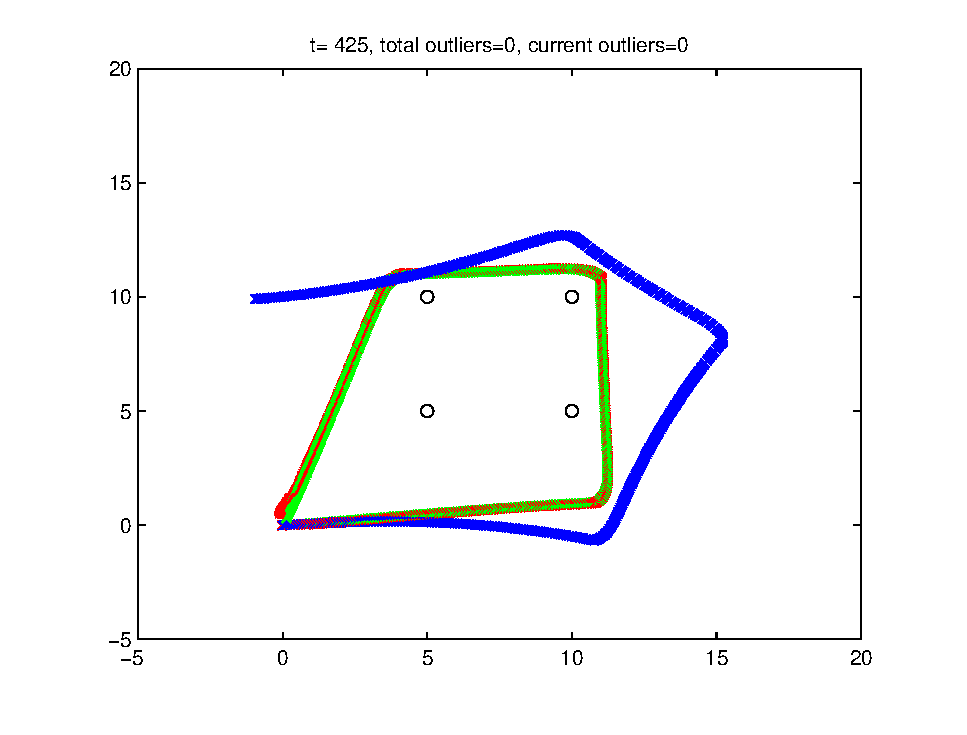
\includegraphics[scale=0.5]{./figures/M=1000/local/1.eps}
	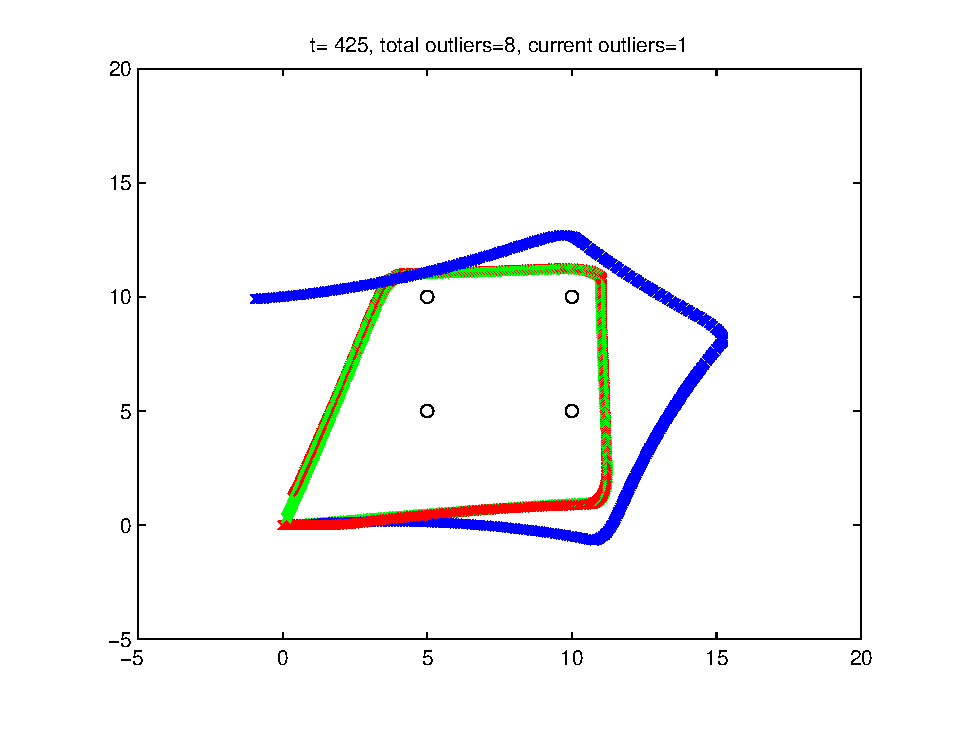
\includegraphics[scale=0.5]{./figures/M=10000/local/1.eps}
	\caption{Resulting trajectories for $M=1000$ (left) and $M=10000$ (right).}
	\label{fig:local_maps_1000_10000}
\end{figure}

\begin{figure}
	\centering
	\scalebox{0.5}{% This file was created by matlab2tikz.
%
%The latest updates can be retrieved from
%  http://www.mathworks.com/matlabcentral/fileexchange/22022-matlab2tikz-matlab2tikz
%where you can also make suggestions and rate matlab2tikz.
%
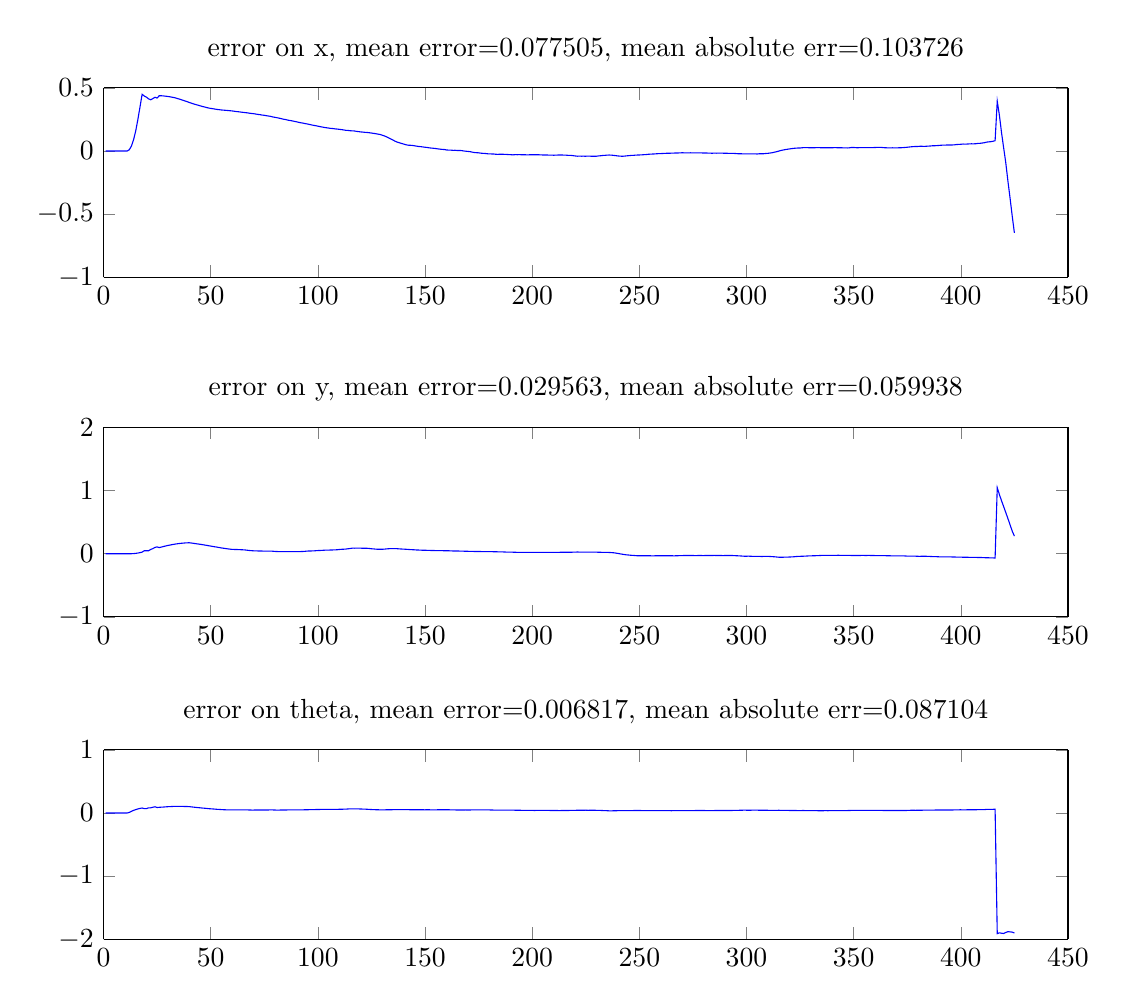
\begin{tikzpicture}

\begin{axis}[%
width=4.822in,
height=0.947in,
at={(0.809in,3.31in)},
scale only axis,
separate axis lines,
every outer x axis line/.append style={black},
every x tick label/.append style={font=\color{black}},
xmin=0,
xmax=450,
every outer y axis line/.append style={black},
every y tick label/.append style={font=\color{black}},
ymin=-1,
ymax=0.5,
axis background/.style={fill=white},
title={error on x, mean error=0.077505, mean absolute err=0.103726}
]
\addplot [color=blue,solid,forget plot]
  table[row sep=crcr]{%
1	0\\
2	0\\
3	0\\
4	0\\
5	0\\
6	0\\
7	0\\
8	0\\
9	0\\
10	0\\
11	0\\
12	0.00955562137445424\\
13	0.0392114902415333\\
14	0.0889396820844108\\
15	0.158714707843808\\
16	0.24851052301998\\
17	0.348779118151642\\
18	0.448990588271203\\
19	0.435665576371415\\
20	0.426386638613298\\
21	0.41323312084001\\
22	0.405570535111214\\
23	0.415423690052686\\
24	0.425647195648471\\
25	0.41932933819804\\
26	0.438241061077142\\
27	0.43744461096412\\
28	0.436068283573504\\
29	0.43402443557718\\
30	0.431880931625316\\
31	0.429308431132644\\
32	0.426047223843889\\
33	0.422942933492238\\
34	0.41822086950343\\
35	0.413041438924649\\
36	0.407777357263298\\
37	0.402068752332956\\
38	0.396309533531984\\
39	0.390649374068324\\
40	0.384449067761939\\
41	0.37873994330238\\
42	0.373016206261361\\
43	0.36794386060948\\
44	0.36339957234887\\
45	0.358401310461349\\
46	0.35325516005693\\
47	0.349158746312148\\
48	0.344720169096946\\
49	0.340602305418412\\
50	0.337413340397827\\
51	0.334970322352831\\
52	0.331897992738868\\
53	0.329111899031455\\
54	0.327362031617947\\
55	0.324873203182057\\
56	0.323642648305071\\
57	0.322213405771855\\
58	0.320839816435678\\
59	0.319061402179902\\
60	0.317436767422851\\
61	0.314817957479482\\
62	0.31250963634038\\
63	0.310899901811436\\
64	0.308434999957021\\
65	0.306326991429127\\
66	0.30427458685454\\
67	0.302438725757622\\
68	0.299652672568901\\
69	0.297531484201622\\
70	0.295503526752664\\
71	0.292805718093564\\
72	0.289812260300543\\
73	0.287838347214463\\
74	0.284734691873258\\
75	0.2828454994902\\
76	0.279469917582126\\
77	0.276875571943353\\
78	0.274484376370387\\
79	0.269559557525994\\
80	0.266677921117892\\
81	0.263399268379731\\
82	0.259858427743471\\
83	0.25582544409336\\
84	0.251656941053591\\
85	0.248932655761976\\
86	0.244534919692444\\
87	0.241671980482481\\
88	0.238599470930703\\
89	0.234916717328583\\
90	0.231462448258341\\
91	0.227376469323073\\
92	0.223788499248625\\
93	0.221106094145662\\
94	0.217429822028773\\
95	0.214307773499717\\
96	0.210712870473911\\
97	0.206791792008868\\
98	0.203242336575057\\
99	0.200485072195162\\
100	0.196627259505142\\
101	0.193215506657154\\
102	0.190033094212229\\
103	0.186781096564292\\
104	0.184134683904849\\
105	0.18173769139235\\
106	0.179165802437637\\
107	0.17795523693189\\
108	0.1752067935225\\
109	0.173778620733589\\
110	0.171811587427811\\
111	0.169561648900068\\
112	0.167017177819268\\
113	0.163915941100944\\
114	0.162981008032816\\
115	0.160665258741082\\
116	0.159652996395314\\
117	0.158666928981948\\
118	0.155733891950412\\
119	0.15347810794699\\
120	0.151144622976801\\
121	0.14976971192584\\
122	0.147829166197601\\
123	0.146796420258486\\
124	0.144691588367255\\
125	0.142258589290547\\
126	0.139557746539811\\
127	0.137135149707021\\
128	0.133772652634052\\
129	0.131138101346448\\
130	0.125457558896898\\
131	0.119587655429115\\
132	0.11235297153017\\
133	0.104131382732575\\
134	0.0956141164263293\\
135	0.0870297334066485\\
136	0.0780346225637452\\
137	0.0701850203243506\\
138	0.0656815081675575\\
139	0.0601817090147012\\
140	0.0551897380336186\\
141	0.0499609186480487\\
142	0.0462178140058942\\
143	0.0455648793092731\\
144	0.0443501091498142\\
145	0.0416809973991459\\
146	0.0387386309000295\\
147	0.0359771428693012\\
148	0.0345908081920854\\
149	0.0321802304786782\\
150	0.0299069067415996\\
151	0.0279479854900888\\
152	0.0250582771060248\\
153	0.0231441408591557\\
154	0.0215046209427907\\
155	0.0194971271929703\\
156	0.016932830617824\\
157	0.0146889943220643\\
158	0.0128237135859131\\
159	0.0117736808716007\\
160	0.00837920114845403\\
161	0.00706799072916198\\
162	0.0069353588993124\\
163	0.00532743590496665\\
164	0.0057594250889359\\
165	0.00405877584465308\\
166	0.00416213281380884\\
167	0.00351013125471944\\
168	0.000525160955719528\\
169	-0.00165606186867251\\
170	-0.00324659923894366\\
171	-0.00517570374900345\\
172	-0.00864719799412406\\
173	-0.0120322439917651\\
174	-0.0132236925551954\\
175	-0.01432906756955\\
176	-0.0169181494825867\\
177	-0.0186307656464759\\
178	-0.019422216188353\\
179	-0.0216640547734421\\
180	-0.0228826490842966\\
181	-0.0232517860229109\\
182	-0.0234235852471336\\
183	-0.0258270658325213\\
184	-0.0264196008799082\\
185	-0.0253711352868127\\
186	-0.0254914926409988\\
187	-0.0264131479232699\\
188	-0.0271633502294932\\
189	-0.0281228020222937\\
190	-0.0291696313398369\\
191	-0.0303556372796816\\
192	-0.0287622454736471\\
193	-0.0292756969203349\\
194	-0.0287866397241228\\
195	-0.0294682900039369\\
196	-0.0292876104351496\\
197	-0.0300173250626408\\
198	-0.0310645050088176\\
199	-0.0291380945707562\\
200	-0.0293775628418942\\
201	-0.0294817155495544\\
202	-0.0295716668199475\\
203	-0.0296736710690801\\
204	-0.0307080636856227\\
205	-0.0314337656899077\\
206	-0.0313337360418959\\
207	-0.0318514206246974\\
208	-0.0324055970135397\\
209	-0.0328141926166836\\
210	-0.0332734466693267\\
211	-0.0328754591400511\\
212	-0.0319168809599883\\
213	-0.0316654129143554\\
214	-0.0317648518025191\\
215	-0.0326529311653161\\
216	-0.033169197488494\\
217	-0.0347532512155926\\
218	-0.0343986909671461\\
219	-0.0367243224295528\\
220	-0.0388334929002294\\
221	-0.041170295084596\\
222	-0.04062463718566\\
223	-0.041115224414968\\
224	-0.0409489604567721\\
225	-0.0412345910567975\\
226	-0.040392955702778\\
227	-0.0408703924843987\\
228	-0.0415988640729736\\
229	-0.0417946308191937\\
230	-0.0410774471549367\\
231	-0.0389098482359582\\
232	-0.0374402471825377\\
233	-0.0352196579848361\\
234	-0.034196746472448\\
235	-0.0323262415602361\\
236	-0.0318870871831134\\
237	-0.0328811512102032\\
238	-0.0346808707828128\\
239	-0.0366819737475659\\
240	-0.0391416919251792\\
241	-0.0404606287102514\\
242	-0.0416604814690995\\
243	-0.0404871201409449\\
244	-0.0384633489327069\\
245	-0.0369856437573137\\
246	-0.0351435998906933\\
247	-0.0346840782029307\\
248	-0.0330037401435366\\
249	-0.0320048934744577\\
250	-0.0312921480410555\\
251	-0.0308511602684902\\
252	-0.0290753751125976\\
253	-0.0284458013294202\\
254	-0.0262996026713864\\
255	-0.0248749669030683\\
256	-0.0240666184553522\\
257	-0.0232357283393547\\
258	-0.0219463304429368\\
259	-0.0207585567018373\\
260	-0.0204039855851832\\
261	-0.0194512758012291\\
262	-0.0183402671464155\\
263	-0.0179621571494586\\
264	-0.0179874138230218\\
265	-0.0167223600056943\\
266	-0.016418063032722\\
267	-0.015808085835781\\
268	-0.0155566578901905\\
269	-0.0147974254932368\\
270	-0.0138118278949921\\
271	-0.0145767141577497\\
272	-0.0142179274780423\\
273	-0.0142239238510582\\
274	-0.0141834192793251\\
275	-0.0146284091755984\\
276	-0.0149879325247113\\
277	-0.0149279501896089\\
278	-0.0152285993117536\\
279	-0.0152079634080629\\
280	-0.0155761493495108\\
281	-0.0154415628439022\\
282	-0.0164686672846388\\
283	-0.0170027937065607\\
284	-0.0175654581058833\\
285	-0.0167975582649564\\
286	-0.0173242494812893\\
287	-0.0163426206633277\\
288	-0.0169887661932675\\
289	-0.0172893812603343\\
290	-0.0174626781962468\\
291	-0.0180615201552632\\
292	-0.0184662158693607\\
293	-0.018296260302578\\
294	-0.0187512428153074\\
295	-0.0200837689169608\\
296	-0.0213946858889997\\
297	-0.0217541441784901\\
298	-0.0221704639394957\\
299	-0.0223510161541256\\
300	-0.0227020554381259\\
301	-0.0222081556185758\\
302	-0.0224547691532484\\
303	-0.0230497211537015\\
304	-0.0225861249615651\\
305	-0.0235976689900097\\
306	-0.0217549403020998\\
307	-0.0219877862679301\\
308	-0.0214099041134865\\
309	-0.0196927566177223\\
310	-0.018312570747578\\
311	-0.0160277499250485\\
312	-0.013498995026739\\
313	-0.00940962913620957\\
314	-0.00552964858768679\\
315	-0.000995041331664837\\
316	0.00408181558323006\\
317	0.00770983868214437\\
318	0.0109443009771657\\
319	0.0137152397756588\\
320	0.0164461060954562\\
321	0.018796828382472\\
322	0.021016238794386\\
323	0.0225207610843454\\
324	0.0237743486923923\\
325	0.02375450377663\\
326	0.0259596624374798\\
327	0.0268180321253491\\
328	0.0271097889630436\\
329	0.0260787329115222\\
330	0.026230197756238\\
331	0.0253812305590482\\
332	0.0262040951457689\\
333	0.0265848497472887\\
334	0.0265584663243121\\
335	0.0256677850244089\\
336	0.0257846471066525\\
337	0.026095379675755\\
338	0.0254014601804666\\
339	0.0259687003238733\\
340	0.0259289059224934\\
341	0.0265223445714722\\
342	0.0262966353783289\\
343	0.0253486697589529\\
344	0.0258619523548478\\
345	0.0252137463945954\\
346	0.0248275205393882\\
347	0.0242568606400066\\
348	0.025267826321095\\
349	0.0280362155916851\\
350	0.0281384291801583\\
351	0.0263348408400796\\
352	0.0260494906504856\\
353	0.0268159103272261\\
354	0.0266245003036203\\
355	0.0269040364271818\\
356	0.0269926273987346\\
357	0.0273224638094702\\
358	0.0269093218178247\\
359	0.027058878922209\\
360	0.0279253754572868\\
361	0.028567712038428\\
362	0.0285587958909184\\
363	0.0282340058078625\\
364	0.0267119459906313\\
365	0.0255291642579323\\
366	0.0251527909283054\\
367	0.0248808104228313\\
368	0.0254515384050025\\
369	0.0251261627986612\\
370	0.0244410855892081\\
371	0.0255690155159203\\
372	0.0258420062292641\\
373	0.0270679473257025\\
374	0.0282523464108302\\
375	0.0298611413532006\\
376	0.0318105490805229\\
377	0.0336451308452839\\
378	0.0351342755915183\\
379	0.0356579562460544\\
380	0.0361514364242843\\
381	0.037539267275762\\
382	0.0373145398268397\\
383	0.0364879985938658\\
384	0.0379103565988466\\
385	0.038892874597489\\
386	0.0400525041069084\\
387	0.0421124243494271\\
388	0.0419533092149051\\
389	0.0430977739509606\\
390	0.0444403500048289\\
391	0.0459472750486776\\
392	0.046596584617095\\
393	0.0469973950933333\\
394	0.0479283628134117\\
395	0.0471331505200681\\
396	0.0478312131583585\\
397	0.0489324130993042\\
398	0.0513978012995161\\
399	0.0523256685480814\\
400	0.0533751619377998\\
401	0.0551549118504223\\
402	0.0548826866723819\\
403	0.0551350082863854\\
404	0.0564354404307549\\
405	0.0571772716441481\\
406	0.0566950824105825\\
407	0.0577404406298712\\
408	0.0603861019091073\\
409	0.0608685420673536\\
410	0.0633270185817429\\
411	0.0657088066599767\\
412	0.070246361667913\\
413	0.0724386402763236\\
414	0.0739271321927358\\
415	0.07708445932222\\
416	0.0818613044672585\\
417	0.394268464142862\\
418	0.284029860482681\\
419	0.145429173534072\\
420	0.0235621123749868\\
421	-0.095795500303318\\
422	-0.241390595480607\\
423	-0.376031097452248\\
424	-0.51675763777199\\
425	-0.648438665990288\\
};
\end{axis}

\begin{axis}[%
width=4.822in,
height=0.947in,
at={(0.809in,1.612in)},
scale only axis,
separate axis lines,
every outer x axis line/.append style={black},
every x tick label/.append style={font=\color{black}},
xmin=0,
xmax=450,
every outer y axis line/.append style={black},
every y tick label/.append style={font=\color{black}},
ymin=-1,
ymax=2,
axis background/.style={fill=white},
title={error on y, mean error=0.029563, mean absolute err=0.059938}
]
\addplot [color=blue,solid,forget plot]
  table[row sep=crcr]{%
1	0\\
2	0\\
3	0\\
4	0\\
5	0\\
6	0\\
7	0\\
8	0\\
9	0\\
10	0\\
11	0\\
12	4.68923517553624e-05\\
13	0.000622000891454959\\
14	0.00236112381575805\\
15	0.00572348872527853\\
16	0.011053629849223\\
17	0.0179379357724753\\
18	0.0255909506065986\\
19	0.047605535859966\\
20	0.0467104321984274\\
21	0.0472152638513229\\
22	0.0683883760158667\\
23	0.0812000474322988\\
24	0.100394010444185\\
25	0.108169250275792\\
26	0.0973352124346576\\
27	0.106257382851095\\
28	0.114991934625321\\
29	0.12328624469211\\
30	0.130819213630006\\
31	0.137687086730886\\
32	0.144422444790804\\
33	0.150711512986103\\
34	0.156012266594144\\
35	0.16087923748531\\
36	0.16454921595292\\
37	0.167948301385888\\
38	0.170895976051161\\
39	0.172918759698165\\
40	0.17419343104948\\
41	0.169652586966969\\
42	0.164871518951504\\
43	0.159574826586946\\
44	0.154999946017788\\
45	0.150217802835201\\
46	0.144785765537998\\
47	0.138716651675221\\
48	0.133495819024522\\
49	0.127222092372599\\
50	0.121601422808288\\
51	0.115416023784177\\
52	0.109726349200436\\
53	0.104315526643053\\
54	0.0979059190513153\\
55	0.092029721431741\\
56	0.0871930909761884\\
57	0.0819943957048241\\
58	0.0771527848467358\\
59	0.0728143562151071\\
60	0.0688845034983552\\
61	0.0679820845046016\\
62	0.0671289969900016\\
63	0.0658217373032199\\
64	0.0640787552329312\\
65	0.0623865223826178\\
66	0.0599910060968039\\
67	0.0557199083034791\\
68	0.0517392832004305\\
69	0.0489512397569173\\
70	0.04643476829575\\
71	0.044685676861245\\
72	0.0443015384759087\\
73	0.0432452145152001\\
74	0.0427372861732911\\
75	0.0414440746148573\\
76	0.0408126030708178\\
77	0.0411721963662172\\
78	0.042074157578616\\
79	0.0398710426389868\\
80	0.0367909705012293\\
81	0.0350159908051499\\
82	0.0338354527369541\\
83	0.0333550867409075\\
84	0.0336782954111664\\
85	0.0336655084949271\\
86	0.0332093108705825\\
87	0.0331018962612869\\
88	0.0330123770826286\\
89	0.0331758490484432\\
90	0.0340050612770113\\
91	0.0341511607677354\\
92	0.0347851358392148\\
93	0.0358869085517795\\
94	0.0385976697243985\\
95	0.0418620077490258\\
96	0.0439003075051783\\
97	0.0442667086475685\\
98	0.0452414027985625\\
99	0.0481889192587985\\
100	0.0506679793093143\\
101	0.0517131877660409\\
102	0.0537697052389117\\
103	0.0559205053666907\\
104	0.0576250647298995\\
105	0.0583596022354709\\
106	0.0586326584850104\\
107	0.060271646890095\\
108	0.0612246177181028\\
109	0.0634217648849238\\
110	0.0674124547243282\\
111	0.0702500666171558\\
112	0.0718860507029477\\
113	0.074142479886158\\
114	0.0787204363905951\\
115	0.0831311773863971\\
116	0.0881111280536199\\
117	0.0878724581467051\\
118	0.0888427042572986\\
119	0.0879844391635958\\
120	0.0880244481072061\\
121	0.087665814379234\\
122	0.0875057838330932\\
123	0.0865439017790072\\
124	0.0832034921404589\\
125	0.0790671789287561\\
126	0.0763275526599085\\
127	0.0730377344021792\\
128	0.0709721725900549\\
129	0.0705876235040698\\
130	0.0710489766627719\\
131	0.0728531978108369\\
132	0.076890906492501\\
133	0.0795885751012038\\
134	0.0810941251839004\\
135	0.0811383236162118\\
136	0.0812811044382218\\
137	0.0799009136276903\\
138	0.0772259291578441\\
139	0.0749308710210517\\
140	0.0730787478747437\\
141	0.0708702775428387\\
142	0.0688310812920245\\
143	0.0659185408389251\\
144	0.0643278686975428\\
145	0.0624850284848057\\
146	0.0596811284285672\\
147	0.0588180993282954\\
148	0.0565460996310438\\
149	0.0556663248066478\\
150	0.0551128194852324\\
151	0.0541402001855795\\
152	0.0530474353655208\\
153	0.0514578851728134\\
154	0.0511478356325434\\
155	0.0497719766787994\\
156	0.0487195957870887\\
157	0.0490341468880007\\
158	0.0485475969874996\\
159	0.0479274094172202\\
160	0.0472202900592786\\
161	0.046875570204036\\
162	0.0461427284494249\\
163	0.0439156620092938\\
164	0.0438762346671897\\
165	0.0433461716965899\\
166	0.0425701112181622\\
167	0.0417091626195569\\
168	0.040498671934893\\
169	0.0394240991806996\\
170	0.0389011639631827\\
171	0.0374628614805257\\
172	0.0370480645980251\\
173	0.03617528487489\\
174	0.0356006009559549\\
175	0.0352857390105976\\
176	0.0349742832868882\\
177	0.0338104626417151\\
178	0.0329185618385566\\
179	0.0335442701254083\\
180	0.0329014987494451\\
181	0.0332651450105246\\
182	0.032112813971465\\
183	0.0316581065643433\\
184	0.0305214880457942\\
185	0.0300209581992101\\
186	0.0299631173135966\\
187	0.0271647549573943\\
188	0.0265139877044032\\
189	0.0258152880772746\\
190	0.0250875666946637\\
191	0.0245169921965873\\
192	0.0236463609863948\\
193	0.0221523463373616\\
194	0.0216641482931781\\
195	0.0215535999480885\\
196	0.0211114283809755\\
197	0.0208840301433346\\
198	0.022029480348813\\
199	0.0219567071104176\\
200	0.0210915996412284\\
201	0.0211019159115988\\
202	0.0216510587331573\\
203	0.0222461441120618\\
204	0.02215852492035\\
205	0.022775667602426\\
206	0.0223152772615407\\
207	0.0226776268387496\\
208	0.0220454105284773\\
209	0.022183164848828\\
210	0.0225329563272396\\
211	0.0219311344501474\\
212	0.0217503745867251\\
213	0.0229485517627523\\
214	0.0230782042165405\\
215	0.0238784138189185\\
216	0.0240952499911433\\
217	0.023186364831373\\
218	0.0233312657117963\\
219	0.0250307010626223\\
220	0.0260749676944343\\
221	0.0270257637114142\\
222	0.0266148502952337\\
223	0.0259814843241202\\
224	0.0258482913320162\\
225	0.0258261111268894\\
226	0.0264608922006317\\
227	0.0267446723288547\\
228	0.0258908783665177\\
229	0.0261323121983335\\
230	0.0250827080926079\\
231	0.0237096638989023\\
232	0.022974021612022\\
233	0.0218724922027196\\
234	0.0217640248008504\\
235	0.0211661924295186\\
236	0.0203059128011827\\
237	0.0178063859324631\\
238	0.0154438358474387\\
239	0.0104115658249846\\
240	0.00521267878915843\\
241	-0.00132398522214494\\
242	-0.00720852787965143\\
243	-0.013129185285397\\
244	-0.0173700286563623\\
245	-0.0204176349057725\\
246	-0.0241229703974017\\
247	-0.0259460522162556\\
248	-0.0291270682168943\\
249	-0.0314763305705412\\
250	-0.0310136463197868\\
251	-0.0323423834979373\\
252	-0.0317913715573361\\
253	-0.0317595596216496\\
254	-0.0319421210096476\\
255	-0.032503137821795\\
256	-0.0327471935264505\\
257	-0.0326566537956481\\
258	-0.0322659889962154\\
259	-0.0322991745588013\\
260	-0.0315757334632831\\
261	-0.0312502222340481\\
262	-0.0318634017667758\\
263	-0.0315120996609757\\
264	-0.0314593334944799\\
265	-0.0316837878831677\\
266	-0.0330393539699187\\
267	-0.0324329478119587\\
268	-0.0311785119557815\\
269	-0.0293492290290267\\
270	-0.0293326198860875\\
271	-0.0278408377342743\\
272	-0.0279788747748011\\
273	-0.0279811675403145\\
274	-0.0281211195452098\\
275	-0.0281145744958948\\
276	-0.02932872020118\\
277	-0.0286629475707656\\
278	-0.0275089727079099\\
279	-0.0284600412894118\\
280	-0.0289729707673594\\
281	-0.0280955495701338\\
282	-0.0279447866912754\\
283	-0.0278728238920891\\
284	-0.0271985801359556\\
285	-0.0267644329184265\\
286	-0.0277569926933516\\
287	-0.0278675215804451\\
288	-0.0278402484473474\\
289	-0.0291555808619339\\
290	-0.0281530360021485\\
291	-0.0279375240867079\\
292	-0.02759652323914\\
293	-0.0275735913302011\\
294	-0.0292257758804713\\
295	-0.0309150498239656\\
296	-0.0325540651024028\\
297	-0.0346112482203491\\
298	-0.0369986183034605\\
299	-0.0393179217772612\\
300	-0.0391855066972955\\
301	-0.0382072218021143\\
302	-0.0399711601715449\\
303	-0.041506825115448\\
304	-0.042423559445055\\
305	-0.0426435175189006\\
306	-0.0425362669470744\\
307	-0.0429309060542487\\
308	-0.0426742641891238\\
309	-0.0426387177398162\\
310	-0.0414913162283934\\
311	-0.0432931992569312\\
312	-0.0455932621799668\\
313	-0.0482277784033442\\
314	-0.0512354259294128\\
315	-0.0547409330052453\\
316	-0.056504078972182\\
317	-0.0547512037576237\\
318	-0.0544627422437358\\
319	-0.0531713741727398\\
320	-0.0518892527341741\\
321	-0.050232837394681\\
322	-0.0481881639564499\\
323	-0.0447496876434794\\
324	-0.0418865713774998\\
325	-0.0408115996800866\\
326	-0.0398142486774979\\
327	-0.0381580547735982\\
328	-0.0364362599739536\\
329	-0.0343951928571808\\
330	-0.0328621497642096\\
331	-0.0324144662366646\\
332	-0.0311511964195628\\
333	-0.0300549843880269\\
334	-0.0285002797697622\\
335	-0.0266323263339654\\
336	-0.0255659174845135\\
337	-0.0247495741020138\\
338	-0.0250320711610907\\
339	-0.0250534540600267\\
340	-0.0252802936398933\\
341	-0.0255715479310687\\
342	-0.0250117943784609\\
343	-0.0242614690108915\\
344	-0.0258184179677006\\
345	-0.0256939336381192\\
346	-0.0252150208713262\\
347	-0.0251248813335927\\
348	-0.0258856117946777\\
349	-0.0276992891248087\\
350	-0.0281163189077125\\
351	-0.0273971544241745\\
352	-0.0276301615300003\\
353	-0.0272207270784222\\
354	-0.0265068959629344\\
355	-0.0269374075652937\\
356	-0.0272225780000284\\
357	-0.0265620913756681\\
358	-0.0272243205635014\\
359	-0.0272723420276719\\
360	-0.0290009621885039\\
361	-0.0299404043024802\\
362	-0.0304430380491771\\
363	-0.0307125606720584\\
364	-0.0306194689299994\\
365	-0.0308709036776502\\
366	-0.0313537168880726\\
367	-0.0324337734932962\\
368	-0.0332363402262583\\
369	-0.0329058154984176\\
370	-0.0334593555802982\\
371	-0.0327332114651702\\
372	-0.0327640783127192\\
373	-0.0332279043972772\\
374	-0.0354354040230893\\
375	-0.0371915852697704\\
376	-0.0377701762463039\\
377	-0.0383589040339931\\
378	-0.0382964122389877\\
379	-0.0388261474452305\\
380	-0.0404833558710926\\
381	-0.040640611800776\\
382	-0.0399551814019947\\
383	-0.0395453702411386\\
384	-0.0404445663412476\\
385	-0.0415713830137339\\
386	-0.0432041372776264\\
387	-0.0451868056801179\\
388	-0.0450010045123492\\
389	-0.0469529219654214\\
390	-0.0488588025959293\\
391	-0.0493129705974624\\
392	-0.0503357644024183\\
393	-0.0503855657771553\\
394	-0.0500398756234182\\
395	-0.049834114314137\\
396	-0.0509652763569051\\
397	-0.0508979690511824\\
398	-0.0533356299923988\\
399	-0.0527698874271039\\
400	-0.0535101626282217\\
401	-0.0552783645768393\\
402	-0.0552360270076799\\
403	-0.0552578444192693\\
404	-0.0574757505090333\\
405	-0.0568120408125607\\
406	-0.0570882417264662\\
407	-0.0581533120973257\\
408	-0.059064974816692\\
409	-0.0588463661568883\\
410	-0.060716053701108\\
411	-0.0620082273078446\\
412	-0.0640457354666766\\
413	-0.0641392595454715\\
414	-0.0650144454845298\\
415	-0.065747137106335\\
416	-0.0681368081206442\\
417	1.04577322851601\\
418	0.938562739659491\\
419	0.838659318763967\\
420	0.746595332053542\\
421	0.651385995591586\\
422	0.555002553560153\\
423	0.457169682709059\\
424	0.357092579072047\\
425	0.279719070485088\\
};
\end{axis}

\begin{axis}[%
width=4.822in,
height=0.947in,
at={(0.809in,0in)},
scale only axis,
separate axis lines,
every outer x axis line/.append style={black},
every x tick label/.append style={font=\color{black}},
xmin=0,
xmax=450,
every outer y axis line/.append style={black},
every y tick label/.append style={font=\color{black}},
ymin=-2,
ymax=1,
axis background/.style={fill=white},
title={error on theta, mean error=0.006817, mean absolute err=0.087104}
]
\addplot [color=blue,solid,forget plot]
  table[row sep=crcr]{%
1	0\\
2	0\\
3	0\\
4	0\\
5	0\\
6	0\\
7	0\\
8	0\\
9	0\\
10	0\\
11	0\\
12	0.00977531043779623\\
13	0.0270356169185559\\
14	0.0416765421666323\\
15	0.0538955052568495\\
16	0.0642116793144671\\
17	0.0727510351741865\\
18	0.0795825528899776\\
19	0.0689656154764076\\
20	0.0696539257530713\\
21	0.0811469332254551\\
22	0.0824757871733963\\
23	0.0915601712151446\\
24	0.0987179137086245\\
25	0.0869050120081116\\
26	0.0902760032884387\\
27	0.0927883237344869\\
28	0.0946004817728974\\
29	0.0973460190464359\\
30	0.100035359283406\\
31	0.101332620886968\\
32	0.103647926365973\\
33	0.10458073625241\\
34	0.105051329392673\\
35	0.105099720263969\\
36	0.105400950425366\\
37	0.104264039771459\\
38	0.103362052661142\\
39	0.102541162598473\\
40	0.101503217846374\\
41	0.096594875152678\\
42	0.093334563261056\\
43	0.0890833048872581\\
44	0.0856539510332204\\
45	0.0827443430565808\\
46	0.0787998618409014\\
47	0.076128555914313\\
48	0.0731563396899286\\
49	0.0687868436190509\\
50	0.0666530374408274\\
51	0.064175212054562\\
52	0.0617746013534846\\
53	0.0580140494081371\\
54	0.0565277114452827\\
55	0.0542648178614247\\
56	0.0522694336471088\\
57	0.0506656779676691\\
58	0.0497926060880411\\
59	0.0492801697206193\\
60	0.048600712928883\\
61	0.0498277098592879\\
62	0.0498806104663139\\
63	0.0500936258260887\\
64	0.0505060096110936\\
65	0.0507593918824338\\
66	0.0506815471210809\\
67	0.0495491854136767\\
68	0.0477802079293608\\
69	0.0468290635420257\\
70	0.0467383417665843\\
71	0.0475080257916405\\
72	0.0481804952112621\\
73	0.0472038145095404\\
74	0.0472675686950925\\
75	0.0478040350257167\\
76	0.0480502768590689\\
77	0.0482697173198017\\
78	0.0498948404458921\\
79	0.0487558903775578\\
80	0.0472624526750627\\
81	0.0459330529485178\\
82	0.0466172489423196\\
83	0.0474162605671489\\
84	0.0479020505575907\\
85	0.0482540849318482\\
86	0.048699848491311\\
87	0.0491678945426535\\
88	0.0498756316223985\\
89	0.049461369218021\\
90	0.0490980012913429\\
91	0.0490590851517063\\
92	0.0498254241070688\\
93	0.0504212434140543\\
94	0.0512219286934723\\
95	0.0520501648569183\\
96	0.0527081302293415\\
97	0.0529757521964216\\
98	0.0532486020845475\\
99	0.0549865758539219\\
100	0.0559538902623373\\
101	0.0564227416615113\\
102	0.057380847814041\\
103	0.0574754870768026\\
104	0.0573389125847439\\
105	0.056980037819077\\
106	0.0567143994198163\\
107	0.0572301392692136\\
108	0.0580509211327334\\
109	0.0579991423147677\\
110	0.0590359151019619\\
111	0.0596167869760893\\
112	0.060611924584951\\
113	0.0609559942141202\\
114	0.0639882227655297\\
115	0.0656869920244851\\
116	0.0663644908412717\\
117	0.0658833165133519\\
118	0.066050137533562\\
119	0.0648290638697531\\
120	0.0637546670784381\\
121	0.0619532630703472\\
122	0.0611641843811563\\
123	0.0593125943241386\\
124	0.0569232392415229\\
125	0.0550074549863546\\
126	0.053550464954772\\
127	0.0523000242601355\\
128	0.0509273778954467\\
129	0.0506687076515067\\
130	0.0506647071202924\\
131	0.0506320718355933\\
132	0.0509066963380036\\
133	0.0517453117800075\\
134	0.052199021635758\\
135	0.0526200002638668\\
136	0.0537678026152917\\
137	0.0529413568774468\\
138	0.0535807931585177\\
139	0.0532730433663127\\
140	0.0541691841209824\\
141	0.0542493936368196\\
142	0.053699303830145\\
143	0.0518596552227866\\
144	0.0509100803693667\\
145	0.0518486588749258\\
146	0.0513125776173124\\
147	0.051081030341745\\
148	0.0509752103660714\\
149	0.051011090800746\\
150	0.0506675294506351\\
151	0.0517917224376943\\
152	0.0512304435796178\\
153	0.0498214111034825\\
154	0.0504496775721606\\
155	0.0502244974026462\\
156	0.0512102992517178\\
157	0.0516121751237288\\
158	0.0512408162388533\\
159	0.0523723393782953\\
160	0.0523439493617808\\
161	0.0519167657620314\\
162	0.0492600303977513\\
163	0.0498540617047718\\
164	0.0486630497897194\\
165	0.0482890940532883\\
166	0.047507209134511\\
167	0.0467813210029169\\
168	0.0475407994069146\\
169	0.0487111070379207\\
170	0.0469659939285285\\
171	0.0480405542900741\\
172	0.0493222727871094\\
173	0.049686558941139\\
174	0.0490877988592962\\
175	0.0486098447637078\\
176	0.0494745879591476\\
177	0.0491290768982635\\
178	0.0489386243612957\\
179	0.0497327533678749\\
180	0.049186906934505\\
181	0.0470064071638543\\
182	0.0468154928280571\\
183	0.0467285699734914\\
184	0.0461666043624409\\
185	0.045740706393727\\
186	0.046184526417635\\
187	0.0452612000193584\\
188	0.0451151030275465\\
189	0.0450560099922952\\
190	0.0451107970764091\\
191	0.045684310284992\\
192	0.0442275128312755\\
193	0.0431649035204504\\
194	0.0435650711935764\\
195	0.0426459434161814\\
196	0.0423425721218669\\
197	0.0425447610858867\\
198	0.041899232880934\\
199	0.0409232384112483\\
200	0.0412305792121508\\
201	0.0403959089426915\\
202	0.0408347382398575\\
203	0.0410981101614878\\
204	0.0406699877794128\\
205	0.0413888526738644\\
206	0.0413804279082779\\
207	0.0409449688844985\\
208	0.0407091190860784\\
209	0.0398849660781178\\
210	0.0400151339533745\\
211	0.0395282264144212\\
212	0.0389462801958027\\
213	0.0387635943996862\\
214	0.0395228068420832\\
215	0.0397225117091615\\
216	0.0399153471840248\\
217	0.0401161751006538\\
218	0.0418603338643173\\
219	0.0415989703043818\\
220	0.0419912242293132\\
221	0.0438984591820404\\
222	0.043176770070156\\
223	0.0439384804919465\\
224	0.0441726157093436\\
225	0.0446507918469452\\
226	0.0426522030416892\\
227	0.0434076941104284\\
228	0.0433795126615752\\
229	0.0436992215573682\\
230	0.042214476097751\\
231	0.0406900418129057\\
232	0.0408253327263646\\
233	0.0387568329752543\\
234	0.0379867125202589\\
235	0.0364454094926194\\
236	0.0341369414600949\\
237	0.0346421790683791\\
238	0.0352686773600537\\
239	0.0354242003981011\\
240	0.0374010831816713\\
241	0.0375395655060125\\
242	0.0384481909079741\\
243	0.0386789510053616\\
244	0.0372105567130578\\
245	0.0370772790983138\\
246	0.0371173077415232\\
247	0.038632389808348\\
248	0.0399145058368298\\
249	0.0401041280497765\\
250	0.0396172329226561\\
251	0.0387709214241436\\
252	0.0388969057191808\\
253	0.0384949288721428\\
254	0.0368599194676165\\
255	0.0374176664011632\\
256	0.0371990126927884\\
257	0.037646484341554\\
258	0.0373807136005109\\
259	0.0368696144681735\\
260	0.0370361627237106\\
261	0.0376139631491057\\
262	0.0372174514975967\\
263	0.0369004323943205\\
264	0.0374263418812593\\
265	0.036350891217082\\
266	0.0380692786284671\\
267	0.03709766545715\\
268	0.0371457871096181\\
269	0.03685896190553\\
270	0.0374783330584982\\
271	0.0374976013854482\\
272	0.0369971734265935\\
273	0.0377677035930013\\
274	0.0377515919248168\\
275	0.0386534401291083\\
276	0.0389515402594878\\
277	0.039138197212055\\
278	0.0393057646726902\\
279	0.0395234233450807\\
280	0.0395889824271656\\
281	0.0386825988706647\\
282	0.038319906839007\\
283	0.0385276397797121\\
284	0.0382986212563381\\
285	0.0389139641848164\\
286	0.0401692318604532\\
287	0.0402535543841109\\
288	0.0404105100060157\\
289	0.0404013168122095\\
290	0.0404787471918038\\
291	0.0402860794755497\\
292	0.0397273764120083\\
293	0.0405341512933433\\
294	0.040712464145189\\
295	0.0407220744543668\\
296	0.0414180002407836\\
297	0.0439466698184763\\
298	0.0441908483132849\\
299	0.0455775349973457\\
300	0.0443322353082714\\
301	0.0441025226257246\\
302	0.044427939609629\\
303	0.045141691093928\\
304	0.0454176539128603\\
305	0.0447030280368876\\
306	0.0444534806827761\\
307	0.0441710279225518\\
308	0.0429474991672851\\
309	0.0430922487255838\\
310	0.0428842971761512\\
311	0.0416140321145519\\
312	0.0415153048090566\\
313	0.0411991777917589\\
314	0.0412549738419967\\
315	0.0433429059930628\\
316	0.0420205147398294\\
317	0.042395473953146\\
318	0.04089277973649\\
319	0.040950180370622\\
320	0.0405160864978669\\
321	0.0398860171741164\\
322	0.0395367788877241\\
323	0.039326239408755\\
324	0.0384280949189053\\
325	0.0377890779186343\\
326	0.0391688465322098\\
327	0.0389689186674858\\
328	0.0377097841217262\\
329	0.0384226645556129\\
330	0.0379082430283688\\
331	0.0376935442541466\\
332	0.0375030253034421\\
333	0.036817599839555\\
334	0.035732017934599\\
335	0.0352577654834336\\
336	0.036606789955278\\
337	0.0372809166154688\\
338	0.0364083000611419\\
339	0.0376305567850395\\
340	0.0368448339410268\\
341	0.0367792455626308\\
342	0.0384295334133853\\
343	0.0377147796826547\\
344	0.0380739728984381\\
345	0.0387372415083629\\
346	0.0381295804115371\\
347	0.03877369260357\\
348	0.0398243276760999\\
349	0.0413570729078812\\
350	0.0407538411088977\\
351	0.0411404973806331\\
352	0.0409903941872241\\
353	0.0417062433069644\\
354	0.041645311761024\\
355	0.0417179540616726\\
356	0.0425349443454239\\
357	0.0424555474360249\\
358	0.0413227294401448\\
359	0.0419259525768094\\
360	0.0423095520078665\\
361	0.0422499234700009\\
362	0.0427234121684608\\
363	0.0418279470592759\\
364	0.039623447063013\\
365	0.0400373927252566\\
366	0.0401565465119376\\
367	0.0396206097294129\\
368	0.0394920059023063\\
369	0.0403591103615071\\
370	0.0403120728446353\\
371	0.0400694005597488\\
372	0.0401727025553749\\
373	0.0393824982805109\\
374	0.0401370089574593\\
375	0.040739372386505\\
376	0.0421515995390367\\
377	0.0437081145657467\\
378	0.0433091323796955\\
379	0.0428142601425296\\
380	0.0434232363263956\\
381	0.0443461145628268\\
382	0.0444581420556194\\
383	0.0451973489974886\\
384	0.046017681607978\\
385	0.0454430529706924\\
386	0.0457788648780353\\
387	0.0466322710131166\\
388	0.0468896338727438\\
389	0.0475482122673014\\
390	0.0474810700387378\\
391	0.0475812067604942\\
392	0.0476512862545553\\
393	0.0480227627986594\\
394	0.0474956731029161\\
395	0.0471282017218879\\
396	0.0479640646789079\\
397	0.0489697722375917\\
398	0.05001988939238\\
399	0.0507119545899268\\
400	0.0509392129780277\\
401	0.0501061224884989\\
402	0.0502456548234331\\
403	0.0509886733680744\\
404	0.0514464164756498\\
405	0.0513671481089659\\
406	0.0516014402831146\\
407	0.0520928477976454\\
408	0.0528645825674783\\
409	0.0532069514990292\\
410	0.0539637749653323\\
411	0.0541808790430691\\
412	0.0568576646283532\\
413	0.0572192722190525\\
414	0.0575362811964411\\
415	0.05827452235068\\
416	0.060250728183183\\
417	-1.91051987719597\\
418	-1.89776828530092\\
419	-1.90381691409292\\
420	-1.9079989677713\\
421	-1.89163238848583\\
422	-1.8791012385805\\
423	-1.88269743839444\\
424	-1.88652180485805\\
425	-1.90080860522801\\
};
\end{axis}
\end{tikzpicture}%}
	\scalebox{0.5}{% This file was created by matlab2tikz.
%
%The latest updates can be retrieved from
%  http://www.mathworks.com/matlabcentral/fileexchange/22022-matlab2tikz-matlab2tikz
%where you can also make suggestions and rate matlab2tikz.
%
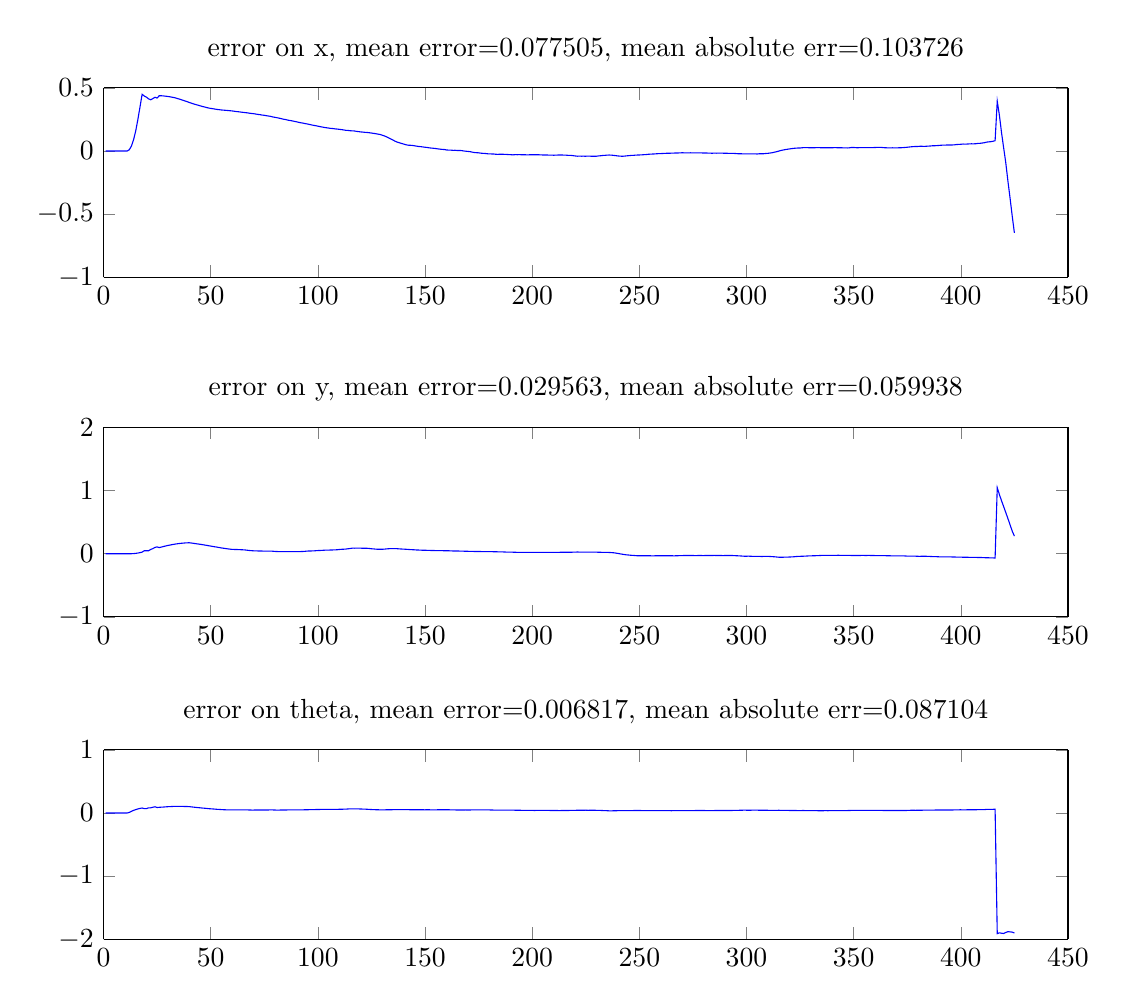
\begin{tikzpicture}

\begin{axis}[%
width=4.822in,
height=0.947in,
at={(0.809in,3.31in)},
scale only axis,
separate axis lines,
every outer x axis line/.append style={black},
every x tick label/.append style={font=\color{black}},
xmin=0,
xmax=450,
every outer y axis line/.append style={black},
every y tick label/.append style={font=\color{black}},
ymin=-1,
ymax=0.5,
axis background/.style={fill=white},
title={error on x, mean error=0.077505, mean absolute err=0.103726}
]
\addplot [color=blue,solid,forget plot]
  table[row sep=crcr]{%
1	0\\
2	0\\
3	0\\
4	0\\
5	0\\
6	0\\
7	0\\
8	0\\
9	0\\
10	0\\
11	0\\
12	0.00955562137445424\\
13	0.0392114902415333\\
14	0.0889396820844108\\
15	0.158714707843808\\
16	0.24851052301998\\
17	0.348779118151642\\
18	0.448990588271203\\
19	0.435665576371415\\
20	0.426386638613298\\
21	0.41323312084001\\
22	0.405570535111214\\
23	0.415423690052686\\
24	0.425647195648471\\
25	0.41932933819804\\
26	0.438241061077142\\
27	0.43744461096412\\
28	0.436068283573504\\
29	0.43402443557718\\
30	0.431880931625316\\
31	0.429308431132644\\
32	0.426047223843889\\
33	0.422942933492238\\
34	0.41822086950343\\
35	0.413041438924649\\
36	0.407777357263298\\
37	0.402068752332956\\
38	0.396309533531984\\
39	0.390649374068324\\
40	0.384449067761939\\
41	0.37873994330238\\
42	0.373016206261361\\
43	0.36794386060948\\
44	0.36339957234887\\
45	0.358401310461349\\
46	0.35325516005693\\
47	0.349158746312148\\
48	0.344720169096946\\
49	0.340602305418412\\
50	0.337413340397827\\
51	0.334970322352831\\
52	0.331897992738868\\
53	0.329111899031455\\
54	0.327362031617947\\
55	0.324873203182057\\
56	0.323642648305071\\
57	0.322213405771855\\
58	0.320839816435678\\
59	0.319061402179902\\
60	0.317436767422851\\
61	0.314817957479482\\
62	0.31250963634038\\
63	0.310899901811436\\
64	0.308434999957021\\
65	0.306326991429127\\
66	0.30427458685454\\
67	0.302438725757622\\
68	0.299652672568901\\
69	0.297531484201622\\
70	0.295503526752664\\
71	0.292805718093564\\
72	0.289812260300543\\
73	0.287838347214463\\
74	0.284734691873258\\
75	0.2828454994902\\
76	0.279469917582126\\
77	0.276875571943353\\
78	0.274484376370387\\
79	0.269559557525994\\
80	0.266677921117892\\
81	0.263399268379731\\
82	0.259858427743471\\
83	0.25582544409336\\
84	0.251656941053591\\
85	0.248932655761976\\
86	0.244534919692444\\
87	0.241671980482481\\
88	0.238599470930703\\
89	0.234916717328583\\
90	0.231462448258341\\
91	0.227376469323073\\
92	0.223788499248625\\
93	0.221106094145662\\
94	0.217429822028773\\
95	0.214307773499717\\
96	0.210712870473911\\
97	0.206791792008868\\
98	0.203242336575057\\
99	0.200485072195162\\
100	0.196627259505142\\
101	0.193215506657154\\
102	0.190033094212229\\
103	0.186781096564292\\
104	0.184134683904849\\
105	0.18173769139235\\
106	0.179165802437637\\
107	0.17795523693189\\
108	0.1752067935225\\
109	0.173778620733589\\
110	0.171811587427811\\
111	0.169561648900068\\
112	0.167017177819268\\
113	0.163915941100944\\
114	0.162981008032816\\
115	0.160665258741082\\
116	0.159652996395314\\
117	0.158666928981948\\
118	0.155733891950412\\
119	0.15347810794699\\
120	0.151144622976801\\
121	0.14976971192584\\
122	0.147829166197601\\
123	0.146796420258486\\
124	0.144691588367255\\
125	0.142258589290547\\
126	0.139557746539811\\
127	0.137135149707021\\
128	0.133772652634052\\
129	0.131138101346448\\
130	0.125457558896898\\
131	0.119587655429115\\
132	0.11235297153017\\
133	0.104131382732575\\
134	0.0956141164263293\\
135	0.0870297334066485\\
136	0.0780346225637452\\
137	0.0701850203243506\\
138	0.0656815081675575\\
139	0.0601817090147012\\
140	0.0551897380336186\\
141	0.0499609186480487\\
142	0.0462178140058942\\
143	0.0455648793092731\\
144	0.0443501091498142\\
145	0.0416809973991459\\
146	0.0387386309000295\\
147	0.0359771428693012\\
148	0.0345908081920854\\
149	0.0321802304786782\\
150	0.0299069067415996\\
151	0.0279479854900888\\
152	0.0250582771060248\\
153	0.0231441408591557\\
154	0.0215046209427907\\
155	0.0194971271929703\\
156	0.016932830617824\\
157	0.0146889943220643\\
158	0.0128237135859131\\
159	0.0117736808716007\\
160	0.00837920114845403\\
161	0.00706799072916198\\
162	0.0069353588993124\\
163	0.00532743590496665\\
164	0.0057594250889359\\
165	0.00405877584465308\\
166	0.00416213281380884\\
167	0.00351013125471944\\
168	0.000525160955719528\\
169	-0.00165606186867251\\
170	-0.00324659923894366\\
171	-0.00517570374900345\\
172	-0.00864719799412406\\
173	-0.0120322439917651\\
174	-0.0132236925551954\\
175	-0.01432906756955\\
176	-0.0169181494825867\\
177	-0.0186307656464759\\
178	-0.019422216188353\\
179	-0.0216640547734421\\
180	-0.0228826490842966\\
181	-0.0232517860229109\\
182	-0.0234235852471336\\
183	-0.0258270658325213\\
184	-0.0264196008799082\\
185	-0.0253711352868127\\
186	-0.0254914926409988\\
187	-0.0264131479232699\\
188	-0.0271633502294932\\
189	-0.0281228020222937\\
190	-0.0291696313398369\\
191	-0.0303556372796816\\
192	-0.0287622454736471\\
193	-0.0292756969203349\\
194	-0.0287866397241228\\
195	-0.0294682900039369\\
196	-0.0292876104351496\\
197	-0.0300173250626408\\
198	-0.0310645050088176\\
199	-0.0291380945707562\\
200	-0.0293775628418942\\
201	-0.0294817155495544\\
202	-0.0295716668199475\\
203	-0.0296736710690801\\
204	-0.0307080636856227\\
205	-0.0314337656899077\\
206	-0.0313337360418959\\
207	-0.0318514206246974\\
208	-0.0324055970135397\\
209	-0.0328141926166836\\
210	-0.0332734466693267\\
211	-0.0328754591400511\\
212	-0.0319168809599883\\
213	-0.0316654129143554\\
214	-0.0317648518025191\\
215	-0.0326529311653161\\
216	-0.033169197488494\\
217	-0.0347532512155926\\
218	-0.0343986909671461\\
219	-0.0367243224295528\\
220	-0.0388334929002294\\
221	-0.041170295084596\\
222	-0.04062463718566\\
223	-0.041115224414968\\
224	-0.0409489604567721\\
225	-0.0412345910567975\\
226	-0.040392955702778\\
227	-0.0408703924843987\\
228	-0.0415988640729736\\
229	-0.0417946308191937\\
230	-0.0410774471549367\\
231	-0.0389098482359582\\
232	-0.0374402471825377\\
233	-0.0352196579848361\\
234	-0.034196746472448\\
235	-0.0323262415602361\\
236	-0.0318870871831134\\
237	-0.0328811512102032\\
238	-0.0346808707828128\\
239	-0.0366819737475659\\
240	-0.0391416919251792\\
241	-0.0404606287102514\\
242	-0.0416604814690995\\
243	-0.0404871201409449\\
244	-0.0384633489327069\\
245	-0.0369856437573137\\
246	-0.0351435998906933\\
247	-0.0346840782029307\\
248	-0.0330037401435366\\
249	-0.0320048934744577\\
250	-0.0312921480410555\\
251	-0.0308511602684902\\
252	-0.0290753751125976\\
253	-0.0284458013294202\\
254	-0.0262996026713864\\
255	-0.0248749669030683\\
256	-0.0240666184553522\\
257	-0.0232357283393547\\
258	-0.0219463304429368\\
259	-0.0207585567018373\\
260	-0.0204039855851832\\
261	-0.0194512758012291\\
262	-0.0183402671464155\\
263	-0.0179621571494586\\
264	-0.0179874138230218\\
265	-0.0167223600056943\\
266	-0.016418063032722\\
267	-0.015808085835781\\
268	-0.0155566578901905\\
269	-0.0147974254932368\\
270	-0.0138118278949921\\
271	-0.0145767141577497\\
272	-0.0142179274780423\\
273	-0.0142239238510582\\
274	-0.0141834192793251\\
275	-0.0146284091755984\\
276	-0.0149879325247113\\
277	-0.0149279501896089\\
278	-0.0152285993117536\\
279	-0.0152079634080629\\
280	-0.0155761493495108\\
281	-0.0154415628439022\\
282	-0.0164686672846388\\
283	-0.0170027937065607\\
284	-0.0175654581058833\\
285	-0.0167975582649564\\
286	-0.0173242494812893\\
287	-0.0163426206633277\\
288	-0.0169887661932675\\
289	-0.0172893812603343\\
290	-0.0174626781962468\\
291	-0.0180615201552632\\
292	-0.0184662158693607\\
293	-0.018296260302578\\
294	-0.0187512428153074\\
295	-0.0200837689169608\\
296	-0.0213946858889997\\
297	-0.0217541441784901\\
298	-0.0221704639394957\\
299	-0.0223510161541256\\
300	-0.0227020554381259\\
301	-0.0222081556185758\\
302	-0.0224547691532484\\
303	-0.0230497211537015\\
304	-0.0225861249615651\\
305	-0.0235976689900097\\
306	-0.0217549403020998\\
307	-0.0219877862679301\\
308	-0.0214099041134865\\
309	-0.0196927566177223\\
310	-0.018312570747578\\
311	-0.0160277499250485\\
312	-0.013498995026739\\
313	-0.00940962913620957\\
314	-0.00552964858768679\\
315	-0.000995041331664837\\
316	0.00408181558323006\\
317	0.00770983868214437\\
318	0.0109443009771657\\
319	0.0137152397756588\\
320	0.0164461060954562\\
321	0.018796828382472\\
322	0.021016238794386\\
323	0.0225207610843454\\
324	0.0237743486923923\\
325	0.02375450377663\\
326	0.0259596624374798\\
327	0.0268180321253491\\
328	0.0271097889630436\\
329	0.0260787329115222\\
330	0.026230197756238\\
331	0.0253812305590482\\
332	0.0262040951457689\\
333	0.0265848497472887\\
334	0.0265584663243121\\
335	0.0256677850244089\\
336	0.0257846471066525\\
337	0.026095379675755\\
338	0.0254014601804666\\
339	0.0259687003238733\\
340	0.0259289059224934\\
341	0.0265223445714722\\
342	0.0262966353783289\\
343	0.0253486697589529\\
344	0.0258619523548478\\
345	0.0252137463945954\\
346	0.0248275205393882\\
347	0.0242568606400066\\
348	0.025267826321095\\
349	0.0280362155916851\\
350	0.0281384291801583\\
351	0.0263348408400796\\
352	0.0260494906504856\\
353	0.0268159103272261\\
354	0.0266245003036203\\
355	0.0269040364271818\\
356	0.0269926273987346\\
357	0.0273224638094702\\
358	0.0269093218178247\\
359	0.027058878922209\\
360	0.0279253754572868\\
361	0.028567712038428\\
362	0.0285587958909184\\
363	0.0282340058078625\\
364	0.0267119459906313\\
365	0.0255291642579323\\
366	0.0251527909283054\\
367	0.0248808104228313\\
368	0.0254515384050025\\
369	0.0251261627986612\\
370	0.0244410855892081\\
371	0.0255690155159203\\
372	0.0258420062292641\\
373	0.0270679473257025\\
374	0.0282523464108302\\
375	0.0298611413532006\\
376	0.0318105490805229\\
377	0.0336451308452839\\
378	0.0351342755915183\\
379	0.0356579562460544\\
380	0.0361514364242843\\
381	0.037539267275762\\
382	0.0373145398268397\\
383	0.0364879985938658\\
384	0.0379103565988466\\
385	0.038892874597489\\
386	0.0400525041069084\\
387	0.0421124243494271\\
388	0.0419533092149051\\
389	0.0430977739509606\\
390	0.0444403500048289\\
391	0.0459472750486776\\
392	0.046596584617095\\
393	0.0469973950933333\\
394	0.0479283628134117\\
395	0.0471331505200681\\
396	0.0478312131583585\\
397	0.0489324130993042\\
398	0.0513978012995161\\
399	0.0523256685480814\\
400	0.0533751619377998\\
401	0.0551549118504223\\
402	0.0548826866723819\\
403	0.0551350082863854\\
404	0.0564354404307549\\
405	0.0571772716441481\\
406	0.0566950824105825\\
407	0.0577404406298712\\
408	0.0603861019091073\\
409	0.0608685420673536\\
410	0.0633270185817429\\
411	0.0657088066599767\\
412	0.070246361667913\\
413	0.0724386402763236\\
414	0.0739271321927358\\
415	0.07708445932222\\
416	0.0818613044672585\\
417	0.394268464142862\\
418	0.284029860482681\\
419	0.145429173534072\\
420	0.0235621123749868\\
421	-0.095795500303318\\
422	-0.241390595480607\\
423	-0.376031097452248\\
424	-0.51675763777199\\
425	-0.648438665990288\\
};
\end{axis}

\begin{axis}[%
width=4.822in,
height=0.947in,
at={(0.809in,1.612in)},
scale only axis,
separate axis lines,
every outer x axis line/.append style={black},
every x tick label/.append style={font=\color{black}},
xmin=0,
xmax=450,
every outer y axis line/.append style={black},
every y tick label/.append style={font=\color{black}},
ymin=-1,
ymax=2,
axis background/.style={fill=white},
title={error on y, mean error=0.029563, mean absolute err=0.059938}
]
\addplot [color=blue,solid,forget plot]
  table[row sep=crcr]{%
1	0\\
2	0\\
3	0\\
4	0\\
5	0\\
6	0\\
7	0\\
8	0\\
9	0\\
10	0\\
11	0\\
12	4.68923517553624e-05\\
13	0.000622000891454959\\
14	0.00236112381575805\\
15	0.00572348872527853\\
16	0.011053629849223\\
17	0.0179379357724753\\
18	0.0255909506065986\\
19	0.047605535859966\\
20	0.0467104321984274\\
21	0.0472152638513229\\
22	0.0683883760158667\\
23	0.0812000474322988\\
24	0.100394010444185\\
25	0.108169250275792\\
26	0.0973352124346576\\
27	0.106257382851095\\
28	0.114991934625321\\
29	0.12328624469211\\
30	0.130819213630006\\
31	0.137687086730886\\
32	0.144422444790804\\
33	0.150711512986103\\
34	0.156012266594144\\
35	0.16087923748531\\
36	0.16454921595292\\
37	0.167948301385888\\
38	0.170895976051161\\
39	0.172918759698165\\
40	0.17419343104948\\
41	0.169652586966969\\
42	0.164871518951504\\
43	0.159574826586946\\
44	0.154999946017788\\
45	0.150217802835201\\
46	0.144785765537998\\
47	0.138716651675221\\
48	0.133495819024522\\
49	0.127222092372599\\
50	0.121601422808288\\
51	0.115416023784177\\
52	0.109726349200436\\
53	0.104315526643053\\
54	0.0979059190513153\\
55	0.092029721431741\\
56	0.0871930909761884\\
57	0.0819943957048241\\
58	0.0771527848467358\\
59	0.0728143562151071\\
60	0.0688845034983552\\
61	0.0679820845046016\\
62	0.0671289969900016\\
63	0.0658217373032199\\
64	0.0640787552329312\\
65	0.0623865223826178\\
66	0.0599910060968039\\
67	0.0557199083034791\\
68	0.0517392832004305\\
69	0.0489512397569173\\
70	0.04643476829575\\
71	0.044685676861245\\
72	0.0443015384759087\\
73	0.0432452145152001\\
74	0.0427372861732911\\
75	0.0414440746148573\\
76	0.0408126030708178\\
77	0.0411721963662172\\
78	0.042074157578616\\
79	0.0398710426389868\\
80	0.0367909705012293\\
81	0.0350159908051499\\
82	0.0338354527369541\\
83	0.0333550867409075\\
84	0.0336782954111664\\
85	0.0336655084949271\\
86	0.0332093108705825\\
87	0.0331018962612869\\
88	0.0330123770826286\\
89	0.0331758490484432\\
90	0.0340050612770113\\
91	0.0341511607677354\\
92	0.0347851358392148\\
93	0.0358869085517795\\
94	0.0385976697243985\\
95	0.0418620077490258\\
96	0.0439003075051783\\
97	0.0442667086475685\\
98	0.0452414027985625\\
99	0.0481889192587985\\
100	0.0506679793093143\\
101	0.0517131877660409\\
102	0.0537697052389117\\
103	0.0559205053666907\\
104	0.0576250647298995\\
105	0.0583596022354709\\
106	0.0586326584850104\\
107	0.060271646890095\\
108	0.0612246177181028\\
109	0.0634217648849238\\
110	0.0674124547243282\\
111	0.0702500666171558\\
112	0.0718860507029477\\
113	0.074142479886158\\
114	0.0787204363905951\\
115	0.0831311773863971\\
116	0.0881111280536199\\
117	0.0878724581467051\\
118	0.0888427042572986\\
119	0.0879844391635958\\
120	0.0880244481072061\\
121	0.087665814379234\\
122	0.0875057838330932\\
123	0.0865439017790072\\
124	0.0832034921404589\\
125	0.0790671789287561\\
126	0.0763275526599085\\
127	0.0730377344021792\\
128	0.0709721725900549\\
129	0.0705876235040698\\
130	0.0710489766627719\\
131	0.0728531978108369\\
132	0.076890906492501\\
133	0.0795885751012038\\
134	0.0810941251839004\\
135	0.0811383236162118\\
136	0.0812811044382218\\
137	0.0799009136276903\\
138	0.0772259291578441\\
139	0.0749308710210517\\
140	0.0730787478747437\\
141	0.0708702775428387\\
142	0.0688310812920245\\
143	0.0659185408389251\\
144	0.0643278686975428\\
145	0.0624850284848057\\
146	0.0596811284285672\\
147	0.0588180993282954\\
148	0.0565460996310438\\
149	0.0556663248066478\\
150	0.0551128194852324\\
151	0.0541402001855795\\
152	0.0530474353655208\\
153	0.0514578851728134\\
154	0.0511478356325434\\
155	0.0497719766787994\\
156	0.0487195957870887\\
157	0.0490341468880007\\
158	0.0485475969874996\\
159	0.0479274094172202\\
160	0.0472202900592786\\
161	0.046875570204036\\
162	0.0461427284494249\\
163	0.0439156620092938\\
164	0.0438762346671897\\
165	0.0433461716965899\\
166	0.0425701112181622\\
167	0.0417091626195569\\
168	0.040498671934893\\
169	0.0394240991806996\\
170	0.0389011639631827\\
171	0.0374628614805257\\
172	0.0370480645980251\\
173	0.03617528487489\\
174	0.0356006009559549\\
175	0.0352857390105976\\
176	0.0349742832868882\\
177	0.0338104626417151\\
178	0.0329185618385566\\
179	0.0335442701254083\\
180	0.0329014987494451\\
181	0.0332651450105246\\
182	0.032112813971465\\
183	0.0316581065643433\\
184	0.0305214880457942\\
185	0.0300209581992101\\
186	0.0299631173135966\\
187	0.0271647549573943\\
188	0.0265139877044032\\
189	0.0258152880772746\\
190	0.0250875666946637\\
191	0.0245169921965873\\
192	0.0236463609863948\\
193	0.0221523463373616\\
194	0.0216641482931781\\
195	0.0215535999480885\\
196	0.0211114283809755\\
197	0.0208840301433346\\
198	0.022029480348813\\
199	0.0219567071104176\\
200	0.0210915996412284\\
201	0.0211019159115988\\
202	0.0216510587331573\\
203	0.0222461441120618\\
204	0.02215852492035\\
205	0.022775667602426\\
206	0.0223152772615407\\
207	0.0226776268387496\\
208	0.0220454105284773\\
209	0.022183164848828\\
210	0.0225329563272396\\
211	0.0219311344501474\\
212	0.0217503745867251\\
213	0.0229485517627523\\
214	0.0230782042165405\\
215	0.0238784138189185\\
216	0.0240952499911433\\
217	0.023186364831373\\
218	0.0233312657117963\\
219	0.0250307010626223\\
220	0.0260749676944343\\
221	0.0270257637114142\\
222	0.0266148502952337\\
223	0.0259814843241202\\
224	0.0258482913320162\\
225	0.0258261111268894\\
226	0.0264608922006317\\
227	0.0267446723288547\\
228	0.0258908783665177\\
229	0.0261323121983335\\
230	0.0250827080926079\\
231	0.0237096638989023\\
232	0.022974021612022\\
233	0.0218724922027196\\
234	0.0217640248008504\\
235	0.0211661924295186\\
236	0.0203059128011827\\
237	0.0178063859324631\\
238	0.0154438358474387\\
239	0.0104115658249846\\
240	0.00521267878915843\\
241	-0.00132398522214494\\
242	-0.00720852787965143\\
243	-0.013129185285397\\
244	-0.0173700286563623\\
245	-0.0204176349057725\\
246	-0.0241229703974017\\
247	-0.0259460522162556\\
248	-0.0291270682168943\\
249	-0.0314763305705412\\
250	-0.0310136463197868\\
251	-0.0323423834979373\\
252	-0.0317913715573361\\
253	-0.0317595596216496\\
254	-0.0319421210096476\\
255	-0.032503137821795\\
256	-0.0327471935264505\\
257	-0.0326566537956481\\
258	-0.0322659889962154\\
259	-0.0322991745588013\\
260	-0.0315757334632831\\
261	-0.0312502222340481\\
262	-0.0318634017667758\\
263	-0.0315120996609757\\
264	-0.0314593334944799\\
265	-0.0316837878831677\\
266	-0.0330393539699187\\
267	-0.0324329478119587\\
268	-0.0311785119557815\\
269	-0.0293492290290267\\
270	-0.0293326198860875\\
271	-0.0278408377342743\\
272	-0.0279788747748011\\
273	-0.0279811675403145\\
274	-0.0281211195452098\\
275	-0.0281145744958948\\
276	-0.02932872020118\\
277	-0.0286629475707656\\
278	-0.0275089727079099\\
279	-0.0284600412894118\\
280	-0.0289729707673594\\
281	-0.0280955495701338\\
282	-0.0279447866912754\\
283	-0.0278728238920891\\
284	-0.0271985801359556\\
285	-0.0267644329184265\\
286	-0.0277569926933516\\
287	-0.0278675215804451\\
288	-0.0278402484473474\\
289	-0.0291555808619339\\
290	-0.0281530360021485\\
291	-0.0279375240867079\\
292	-0.02759652323914\\
293	-0.0275735913302011\\
294	-0.0292257758804713\\
295	-0.0309150498239656\\
296	-0.0325540651024028\\
297	-0.0346112482203491\\
298	-0.0369986183034605\\
299	-0.0393179217772612\\
300	-0.0391855066972955\\
301	-0.0382072218021143\\
302	-0.0399711601715449\\
303	-0.041506825115448\\
304	-0.042423559445055\\
305	-0.0426435175189006\\
306	-0.0425362669470744\\
307	-0.0429309060542487\\
308	-0.0426742641891238\\
309	-0.0426387177398162\\
310	-0.0414913162283934\\
311	-0.0432931992569312\\
312	-0.0455932621799668\\
313	-0.0482277784033442\\
314	-0.0512354259294128\\
315	-0.0547409330052453\\
316	-0.056504078972182\\
317	-0.0547512037576237\\
318	-0.0544627422437358\\
319	-0.0531713741727398\\
320	-0.0518892527341741\\
321	-0.050232837394681\\
322	-0.0481881639564499\\
323	-0.0447496876434794\\
324	-0.0418865713774998\\
325	-0.0408115996800866\\
326	-0.0398142486774979\\
327	-0.0381580547735982\\
328	-0.0364362599739536\\
329	-0.0343951928571808\\
330	-0.0328621497642096\\
331	-0.0324144662366646\\
332	-0.0311511964195628\\
333	-0.0300549843880269\\
334	-0.0285002797697622\\
335	-0.0266323263339654\\
336	-0.0255659174845135\\
337	-0.0247495741020138\\
338	-0.0250320711610907\\
339	-0.0250534540600267\\
340	-0.0252802936398933\\
341	-0.0255715479310687\\
342	-0.0250117943784609\\
343	-0.0242614690108915\\
344	-0.0258184179677006\\
345	-0.0256939336381192\\
346	-0.0252150208713262\\
347	-0.0251248813335927\\
348	-0.0258856117946777\\
349	-0.0276992891248087\\
350	-0.0281163189077125\\
351	-0.0273971544241745\\
352	-0.0276301615300003\\
353	-0.0272207270784222\\
354	-0.0265068959629344\\
355	-0.0269374075652937\\
356	-0.0272225780000284\\
357	-0.0265620913756681\\
358	-0.0272243205635014\\
359	-0.0272723420276719\\
360	-0.0290009621885039\\
361	-0.0299404043024802\\
362	-0.0304430380491771\\
363	-0.0307125606720584\\
364	-0.0306194689299994\\
365	-0.0308709036776502\\
366	-0.0313537168880726\\
367	-0.0324337734932962\\
368	-0.0332363402262583\\
369	-0.0329058154984176\\
370	-0.0334593555802982\\
371	-0.0327332114651702\\
372	-0.0327640783127192\\
373	-0.0332279043972772\\
374	-0.0354354040230893\\
375	-0.0371915852697704\\
376	-0.0377701762463039\\
377	-0.0383589040339931\\
378	-0.0382964122389877\\
379	-0.0388261474452305\\
380	-0.0404833558710926\\
381	-0.040640611800776\\
382	-0.0399551814019947\\
383	-0.0395453702411386\\
384	-0.0404445663412476\\
385	-0.0415713830137339\\
386	-0.0432041372776264\\
387	-0.0451868056801179\\
388	-0.0450010045123492\\
389	-0.0469529219654214\\
390	-0.0488588025959293\\
391	-0.0493129705974624\\
392	-0.0503357644024183\\
393	-0.0503855657771553\\
394	-0.0500398756234182\\
395	-0.049834114314137\\
396	-0.0509652763569051\\
397	-0.0508979690511824\\
398	-0.0533356299923988\\
399	-0.0527698874271039\\
400	-0.0535101626282217\\
401	-0.0552783645768393\\
402	-0.0552360270076799\\
403	-0.0552578444192693\\
404	-0.0574757505090333\\
405	-0.0568120408125607\\
406	-0.0570882417264662\\
407	-0.0581533120973257\\
408	-0.059064974816692\\
409	-0.0588463661568883\\
410	-0.060716053701108\\
411	-0.0620082273078446\\
412	-0.0640457354666766\\
413	-0.0641392595454715\\
414	-0.0650144454845298\\
415	-0.065747137106335\\
416	-0.0681368081206442\\
417	1.04577322851601\\
418	0.938562739659491\\
419	0.838659318763967\\
420	0.746595332053542\\
421	0.651385995591586\\
422	0.555002553560153\\
423	0.457169682709059\\
424	0.357092579072047\\
425	0.279719070485088\\
};
\end{axis}

\begin{axis}[%
width=4.822in,
height=0.947in,
at={(0.809in,0in)},
scale only axis,
separate axis lines,
every outer x axis line/.append style={black},
every x tick label/.append style={font=\color{black}},
xmin=0,
xmax=450,
every outer y axis line/.append style={black},
every y tick label/.append style={font=\color{black}},
ymin=-2,
ymax=1,
axis background/.style={fill=white},
title={error on theta, mean error=0.006817, mean absolute err=0.087104}
]
\addplot [color=blue,solid,forget plot]
  table[row sep=crcr]{%
1	0\\
2	0\\
3	0\\
4	0\\
5	0\\
6	0\\
7	0\\
8	0\\
9	0\\
10	0\\
11	0\\
12	0.00977531043779623\\
13	0.0270356169185559\\
14	0.0416765421666323\\
15	0.0538955052568495\\
16	0.0642116793144671\\
17	0.0727510351741865\\
18	0.0795825528899776\\
19	0.0689656154764076\\
20	0.0696539257530713\\
21	0.0811469332254551\\
22	0.0824757871733963\\
23	0.0915601712151446\\
24	0.0987179137086245\\
25	0.0869050120081116\\
26	0.0902760032884387\\
27	0.0927883237344869\\
28	0.0946004817728974\\
29	0.0973460190464359\\
30	0.100035359283406\\
31	0.101332620886968\\
32	0.103647926365973\\
33	0.10458073625241\\
34	0.105051329392673\\
35	0.105099720263969\\
36	0.105400950425366\\
37	0.104264039771459\\
38	0.103362052661142\\
39	0.102541162598473\\
40	0.101503217846374\\
41	0.096594875152678\\
42	0.093334563261056\\
43	0.0890833048872581\\
44	0.0856539510332204\\
45	0.0827443430565808\\
46	0.0787998618409014\\
47	0.076128555914313\\
48	0.0731563396899286\\
49	0.0687868436190509\\
50	0.0666530374408274\\
51	0.064175212054562\\
52	0.0617746013534846\\
53	0.0580140494081371\\
54	0.0565277114452827\\
55	0.0542648178614247\\
56	0.0522694336471088\\
57	0.0506656779676691\\
58	0.0497926060880411\\
59	0.0492801697206193\\
60	0.048600712928883\\
61	0.0498277098592879\\
62	0.0498806104663139\\
63	0.0500936258260887\\
64	0.0505060096110936\\
65	0.0507593918824338\\
66	0.0506815471210809\\
67	0.0495491854136767\\
68	0.0477802079293608\\
69	0.0468290635420257\\
70	0.0467383417665843\\
71	0.0475080257916405\\
72	0.0481804952112621\\
73	0.0472038145095404\\
74	0.0472675686950925\\
75	0.0478040350257167\\
76	0.0480502768590689\\
77	0.0482697173198017\\
78	0.0498948404458921\\
79	0.0487558903775578\\
80	0.0472624526750627\\
81	0.0459330529485178\\
82	0.0466172489423196\\
83	0.0474162605671489\\
84	0.0479020505575907\\
85	0.0482540849318482\\
86	0.048699848491311\\
87	0.0491678945426535\\
88	0.0498756316223985\\
89	0.049461369218021\\
90	0.0490980012913429\\
91	0.0490590851517063\\
92	0.0498254241070688\\
93	0.0504212434140543\\
94	0.0512219286934723\\
95	0.0520501648569183\\
96	0.0527081302293415\\
97	0.0529757521964216\\
98	0.0532486020845475\\
99	0.0549865758539219\\
100	0.0559538902623373\\
101	0.0564227416615113\\
102	0.057380847814041\\
103	0.0574754870768026\\
104	0.0573389125847439\\
105	0.056980037819077\\
106	0.0567143994198163\\
107	0.0572301392692136\\
108	0.0580509211327334\\
109	0.0579991423147677\\
110	0.0590359151019619\\
111	0.0596167869760893\\
112	0.060611924584951\\
113	0.0609559942141202\\
114	0.0639882227655297\\
115	0.0656869920244851\\
116	0.0663644908412717\\
117	0.0658833165133519\\
118	0.066050137533562\\
119	0.0648290638697531\\
120	0.0637546670784381\\
121	0.0619532630703472\\
122	0.0611641843811563\\
123	0.0593125943241386\\
124	0.0569232392415229\\
125	0.0550074549863546\\
126	0.053550464954772\\
127	0.0523000242601355\\
128	0.0509273778954467\\
129	0.0506687076515067\\
130	0.0506647071202924\\
131	0.0506320718355933\\
132	0.0509066963380036\\
133	0.0517453117800075\\
134	0.052199021635758\\
135	0.0526200002638668\\
136	0.0537678026152917\\
137	0.0529413568774468\\
138	0.0535807931585177\\
139	0.0532730433663127\\
140	0.0541691841209824\\
141	0.0542493936368196\\
142	0.053699303830145\\
143	0.0518596552227866\\
144	0.0509100803693667\\
145	0.0518486588749258\\
146	0.0513125776173124\\
147	0.051081030341745\\
148	0.0509752103660714\\
149	0.051011090800746\\
150	0.0506675294506351\\
151	0.0517917224376943\\
152	0.0512304435796178\\
153	0.0498214111034825\\
154	0.0504496775721606\\
155	0.0502244974026462\\
156	0.0512102992517178\\
157	0.0516121751237288\\
158	0.0512408162388533\\
159	0.0523723393782953\\
160	0.0523439493617808\\
161	0.0519167657620314\\
162	0.0492600303977513\\
163	0.0498540617047718\\
164	0.0486630497897194\\
165	0.0482890940532883\\
166	0.047507209134511\\
167	0.0467813210029169\\
168	0.0475407994069146\\
169	0.0487111070379207\\
170	0.0469659939285285\\
171	0.0480405542900741\\
172	0.0493222727871094\\
173	0.049686558941139\\
174	0.0490877988592962\\
175	0.0486098447637078\\
176	0.0494745879591476\\
177	0.0491290768982635\\
178	0.0489386243612957\\
179	0.0497327533678749\\
180	0.049186906934505\\
181	0.0470064071638543\\
182	0.0468154928280571\\
183	0.0467285699734914\\
184	0.0461666043624409\\
185	0.045740706393727\\
186	0.046184526417635\\
187	0.0452612000193584\\
188	0.0451151030275465\\
189	0.0450560099922952\\
190	0.0451107970764091\\
191	0.045684310284992\\
192	0.0442275128312755\\
193	0.0431649035204504\\
194	0.0435650711935764\\
195	0.0426459434161814\\
196	0.0423425721218669\\
197	0.0425447610858867\\
198	0.041899232880934\\
199	0.0409232384112483\\
200	0.0412305792121508\\
201	0.0403959089426915\\
202	0.0408347382398575\\
203	0.0410981101614878\\
204	0.0406699877794128\\
205	0.0413888526738644\\
206	0.0413804279082779\\
207	0.0409449688844985\\
208	0.0407091190860784\\
209	0.0398849660781178\\
210	0.0400151339533745\\
211	0.0395282264144212\\
212	0.0389462801958027\\
213	0.0387635943996862\\
214	0.0395228068420832\\
215	0.0397225117091615\\
216	0.0399153471840248\\
217	0.0401161751006538\\
218	0.0418603338643173\\
219	0.0415989703043818\\
220	0.0419912242293132\\
221	0.0438984591820404\\
222	0.043176770070156\\
223	0.0439384804919465\\
224	0.0441726157093436\\
225	0.0446507918469452\\
226	0.0426522030416892\\
227	0.0434076941104284\\
228	0.0433795126615752\\
229	0.0436992215573682\\
230	0.042214476097751\\
231	0.0406900418129057\\
232	0.0408253327263646\\
233	0.0387568329752543\\
234	0.0379867125202589\\
235	0.0364454094926194\\
236	0.0341369414600949\\
237	0.0346421790683791\\
238	0.0352686773600537\\
239	0.0354242003981011\\
240	0.0374010831816713\\
241	0.0375395655060125\\
242	0.0384481909079741\\
243	0.0386789510053616\\
244	0.0372105567130578\\
245	0.0370772790983138\\
246	0.0371173077415232\\
247	0.038632389808348\\
248	0.0399145058368298\\
249	0.0401041280497765\\
250	0.0396172329226561\\
251	0.0387709214241436\\
252	0.0388969057191808\\
253	0.0384949288721428\\
254	0.0368599194676165\\
255	0.0374176664011632\\
256	0.0371990126927884\\
257	0.037646484341554\\
258	0.0373807136005109\\
259	0.0368696144681735\\
260	0.0370361627237106\\
261	0.0376139631491057\\
262	0.0372174514975967\\
263	0.0369004323943205\\
264	0.0374263418812593\\
265	0.036350891217082\\
266	0.0380692786284671\\
267	0.03709766545715\\
268	0.0371457871096181\\
269	0.03685896190553\\
270	0.0374783330584982\\
271	0.0374976013854482\\
272	0.0369971734265935\\
273	0.0377677035930013\\
274	0.0377515919248168\\
275	0.0386534401291083\\
276	0.0389515402594878\\
277	0.039138197212055\\
278	0.0393057646726902\\
279	0.0395234233450807\\
280	0.0395889824271656\\
281	0.0386825988706647\\
282	0.038319906839007\\
283	0.0385276397797121\\
284	0.0382986212563381\\
285	0.0389139641848164\\
286	0.0401692318604532\\
287	0.0402535543841109\\
288	0.0404105100060157\\
289	0.0404013168122095\\
290	0.0404787471918038\\
291	0.0402860794755497\\
292	0.0397273764120083\\
293	0.0405341512933433\\
294	0.040712464145189\\
295	0.0407220744543668\\
296	0.0414180002407836\\
297	0.0439466698184763\\
298	0.0441908483132849\\
299	0.0455775349973457\\
300	0.0443322353082714\\
301	0.0441025226257246\\
302	0.044427939609629\\
303	0.045141691093928\\
304	0.0454176539128603\\
305	0.0447030280368876\\
306	0.0444534806827761\\
307	0.0441710279225518\\
308	0.0429474991672851\\
309	0.0430922487255838\\
310	0.0428842971761512\\
311	0.0416140321145519\\
312	0.0415153048090566\\
313	0.0411991777917589\\
314	0.0412549738419967\\
315	0.0433429059930628\\
316	0.0420205147398294\\
317	0.042395473953146\\
318	0.04089277973649\\
319	0.040950180370622\\
320	0.0405160864978669\\
321	0.0398860171741164\\
322	0.0395367788877241\\
323	0.039326239408755\\
324	0.0384280949189053\\
325	0.0377890779186343\\
326	0.0391688465322098\\
327	0.0389689186674858\\
328	0.0377097841217262\\
329	0.0384226645556129\\
330	0.0379082430283688\\
331	0.0376935442541466\\
332	0.0375030253034421\\
333	0.036817599839555\\
334	0.035732017934599\\
335	0.0352577654834336\\
336	0.036606789955278\\
337	0.0372809166154688\\
338	0.0364083000611419\\
339	0.0376305567850395\\
340	0.0368448339410268\\
341	0.0367792455626308\\
342	0.0384295334133853\\
343	0.0377147796826547\\
344	0.0380739728984381\\
345	0.0387372415083629\\
346	0.0381295804115371\\
347	0.03877369260357\\
348	0.0398243276760999\\
349	0.0413570729078812\\
350	0.0407538411088977\\
351	0.0411404973806331\\
352	0.0409903941872241\\
353	0.0417062433069644\\
354	0.041645311761024\\
355	0.0417179540616726\\
356	0.0425349443454239\\
357	0.0424555474360249\\
358	0.0413227294401448\\
359	0.0419259525768094\\
360	0.0423095520078665\\
361	0.0422499234700009\\
362	0.0427234121684608\\
363	0.0418279470592759\\
364	0.039623447063013\\
365	0.0400373927252566\\
366	0.0401565465119376\\
367	0.0396206097294129\\
368	0.0394920059023063\\
369	0.0403591103615071\\
370	0.0403120728446353\\
371	0.0400694005597488\\
372	0.0401727025553749\\
373	0.0393824982805109\\
374	0.0401370089574593\\
375	0.040739372386505\\
376	0.0421515995390367\\
377	0.0437081145657467\\
378	0.0433091323796955\\
379	0.0428142601425296\\
380	0.0434232363263956\\
381	0.0443461145628268\\
382	0.0444581420556194\\
383	0.0451973489974886\\
384	0.046017681607978\\
385	0.0454430529706924\\
386	0.0457788648780353\\
387	0.0466322710131166\\
388	0.0468896338727438\\
389	0.0475482122673014\\
390	0.0474810700387378\\
391	0.0475812067604942\\
392	0.0476512862545553\\
393	0.0480227627986594\\
394	0.0474956731029161\\
395	0.0471282017218879\\
396	0.0479640646789079\\
397	0.0489697722375917\\
398	0.05001988939238\\
399	0.0507119545899268\\
400	0.0509392129780277\\
401	0.0501061224884989\\
402	0.0502456548234331\\
403	0.0509886733680744\\
404	0.0514464164756498\\
405	0.0513671481089659\\
406	0.0516014402831146\\
407	0.0520928477976454\\
408	0.0528645825674783\\
409	0.0532069514990292\\
410	0.0539637749653323\\
411	0.0541808790430691\\
412	0.0568576646283532\\
413	0.0572192722190525\\
414	0.0575362811964411\\
415	0.05827452235068\\
416	0.060250728183183\\
417	-1.91051987719597\\
418	-1.89776828530092\\
419	-1.90381691409292\\
420	-1.9079989677713\\
421	-1.89163238848583\\
422	-1.8791012385805\\
423	-1.88269743839444\\
424	-1.88652180485805\\
425	-1.90080860522801\\
};
\end{axis}
\end{tikzpicture}%}
	\caption{Mean pose errors for $M=1000$ (left) and $M=10000$ (right).}
	\label{fig:local_errors_1000_10000}
\end{figure}

\begin{figure}
	\centering
	\scalebox{0.5}{% This file was created by matlab2tikz.
%
%The latest updates can be retrieved from
%  http://www.mathworks.com/matlabcentral/fileexchange/22022-matlab2tikz-matlab2tikz
%where you can also make suggestions and rate matlab2tikz.
%
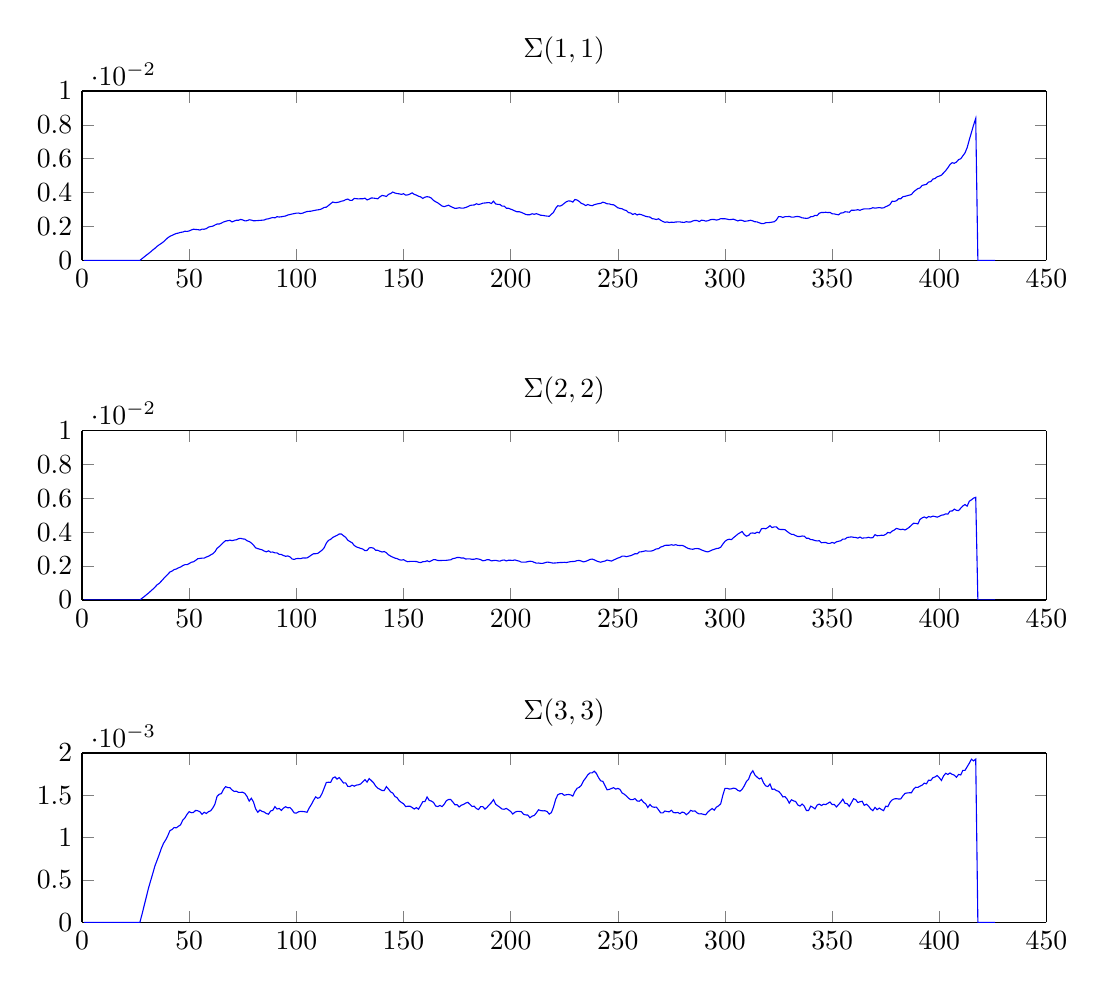
\begin{tikzpicture}

\begin{axis}[%
width=4.822in,
height=0.847in,
at={(0.809in,3.31in)},
scale only axis,
separate axis lines,
every outer x axis line/.append style={black},
every x tick label/.append style={font=\color{black}},
xmin=0,
xmax=450,
every outer y axis line/.append style={black},
every y tick label/.append style={font=\color{black}},
ymin=0,
ymax=0.01,
axis background/.style={fill=white},
title={$\Sigma\text{(1,1)}$}
]
\addplot [color=blue,solid,forget plot]
  table[row sep=crcr]{%
1	0\\
2	0\\
3	0\\
4	0\\
5	0\\
6	0\\
7	0\\
8	0\\
9	0\\
10	0\\
11	0\\
12	0\\
13	0\\
14	0\\
15	0\\
16	0\\
17	0\\
18	0\\
19	0\\
20	1.10668068063497e-28\\
21	6.1269188077788e-29\\
22	1.21154341531275e-27\\
23	2.16417281386742e-27\\
24	6.14431246491431e-27\\
25	6.28434927927247e-27\\
26	6.73213425124081e-27\\
27	5.07990940394863e-28\\
28	0.000100848759663641\\
29	0.00020187458630563\\
30	0.000305214346819941\\
31	0.000398660148707806\\
32	0.000499726900089777\\
33	0.00061192158000982\\
34	0.000708930345163692\\
35	0.000827918770452437\\
36	0.00091868681683618\\
37	0.00100197044500345\\
38	0.00109437218641779\\
39	0.00121342497173134\\
40	0.00133195545626767\\
41	0.00141823104363627\\
42	0.00147534380135983\\
43	0.00153731462564227\\
44	0.00158465558470437\\
45	0.00161161690715752\\
46	0.00165206093191761\\
47	0.00166981777931582\\
48	0.00171804000766001\\
49	0.00170631699294439\\
50	0.00173851789157291\\
51	0.00179223648974585\\
52	0.00183936471620231\\
53	0.00182310648097971\\
54	0.00181498429416863\\
55	0.00178917674870309\\
56	0.00183994667323329\\
57	0.00183880120246031\\
58	0.00187236753121147\\
59	0.00196158996028609\\
60	0.00199432071828742\\
61	0.00201714297453399\\
62	0.00208460294759297\\
63	0.00214652306975963\\
64	0.00214265193310957\\
65	0.00219868508884968\\
66	0.00226426280496353\\
67	0.00230408818126919\\
68	0.0023408784342245\\
69	0.00235403209879532\\
70	0.00226827797836073\\
71	0.00232033446250976\\
72	0.00236911589104423\\
73	0.002365903289477\\
74	0.0024171892358195\\
75	0.00238586112474731\\
76	0.00232927765645765\\
77	0.00234149551120929\\
78	0.00239405169022441\\
79	0.00237777287871326\\
80	0.00233320489064618\\
81	0.00234151787734478\\
82	0.00234948408204308\\
83	0.00235944604561368\\
84	0.0023699385354519\\
85	0.00238191501583074\\
86	0.00243532228243168\\
87	0.00245332531953899\\
88	0.00249787718767231\\
89	0.00252682422052829\\
90	0.00251095190728026\\
91	0.00257744077134686\\
92	0.00255862456799322\\
93	0.00257329973758199\\
94	0.0025964145974395\\
95	0.00261983730191888\\
96	0.00267576439870782\\
97	0.00270363472710814\\
98	0.00273540525674294\\
99	0.00276067516512187\\
100	0.00278631074366188\\
101	0.00279233327817584\\
102	0.00276275022841953\\
103	0.00278865765676907\\
104	0.00284144709007201\\
105	0.00288280220871039\\
106	0.00289431325542503\\
107	0.0029046595732406\\
108	0.00293621878515766\\
109	0.00296127253800892\\
110	0.00298144365824422\\
111	0.00300197408752758\\
112	0.00304853956320662\\
113	0.00312738246397327\\
114	0.00313752844144664\\
115	0.00323995894700459\\
116	0.00334426486425147\\
117	0.00344330092484347\\
118	0.00340927013385469\\
119	0.00341733958671464\\
120	0.00344580903204775\\
121	0.00349192413918856\\
122	0.00351637763763639\\
123	0.00358221663619034\\
124	0.00361705091063439\\
125	0.0035436681607256\\
126	0.00354119616168422\\
127	0.0036529348867921\\
128	0.00364123727188945\\
129	0.003626852367933\\
130	0.00363783043905127\\
131	0.00363251396216881\\
132	0.00367344457001959\\
133	0.00356800291719922\\
134	0.00361325887447694\\
135	0.00368506220515819\\
136	0.00367453225551926\\
137	0.00365665373707\\
138	0.00363466810309075\\
139	0.0037509007557095\\
140	0.00383212035603466\\
141	0.00380973917925498\\
142	0.0037728854319384\\
143	0.00389388972526819\\
144	0.00394511636830079\\
145	0.00403256666484179\\
146	0.00397428300900783\\
147	0.00394277203690242\\
148	0.0039267521983077\\
149	0.00389409260409789\\
150	0.00393183027997855\\
151	0.00385070532229674\\
152	0.00386387169272818\\
153	0.00391435810966989\\
154	0.00398516930076559\\
155	0.00389521188821937\\
156	0.00385464520089499\\
157	0.00378587264207597\\
158	0.00374943798269655\\
159	0.00365622475233085\\
160	0.00373113035666882\\
161	0.00375880836109623\\
162	0.00373744149184959\\
163	0.00367190667563139\\
164	0.0035382154659741\\
165	0.00346171558808308\\
166	0.00339279018079965\\
167	0.00329994637304831\\
168	0.00320698079219232\\
169	0.00316911963246575\\
170	0.00321136256350379\\
171	0.00325581854841401\\
172	0.00318083539976905\\
173	0.00312403689446414\\
174	0.00306927534170966\\
175	0.00307801036982269\\
176	0.0031067814948014\\
177	0.00308267425073142\\
178	0.00308521063868562\\
179	0.00312071836267238\\
180	0.00316907108981676\\
181	0.00323735917622743\\
182	0.00326140044617571\\
183	0.0032669441160519\\
184	0.00334048681538286\\
185	0.00329794248103543\\
186	0.00332671759036052\\
187	0.00337396268442482\\
188	0.00338666859837515\\
189	0.00340301556506458\\
190	0.00341065571121403\\
191	0.00335540547875238\\
192	0.00349252741341112\\
193	0.00333132426594948\\
194	0.00330207179669148\\
195	0.0032985388514196\\
196	0.00320242889181633\\
197	0.00319601154911751\\
198	0.00307514549851362\\
199	0.00307477024042898\\
200	0.00302247293532463\\
201	0.00297537751101938\\
202	0.00291477690550335\\
203	0.00286461940120865\\
204	0.00287415118853271\\
205	0.0028301426446641\\
206	0.00277349706618181\\
207	0.00271072448634254\\
208	0.00268867243669324\\
209	0.00269340681839635\\
210	0.00275209560572301\\
211	0.00271741746342264\\
212	0.00275733382987517\\
213	0.00271144055892187\\
214	0.00266378446039729\\
215	0.00265237171957067\\
216	0.00262965062063816\\
217	0.00261164909910056\\
218	0.00260043668310072\\
219	0.00272049309242529\\
220	0.00283304822372427\\
221	0.00307734942174367\\
222	0.00322628078786898\\
223	0.00320004568578852\\
224	0.00326173375686092\\
225	0.00336393498011407\\
226	0.00345820530964664\\
227	0.00351023494096158\\
228	0.00349817005547822\\
229	0.00343877432271297\\
230	0.00359610133657647\\
231	0.00355797273417922\\
232	0.0034777240401972\\
233	0.00336273886208658\\
234	0.00331824633399705\\
235	0.0032336949960527\\
236	0.00329751175641192\\
237	0.00325012762354946\\
238	0.00322694639863512\\
239	0.00328326790187974\\
240	0.00331957731045358\\
241	0.00334860372720795\\
242	0.00336579111464971\\
243	0.0034328540094083\\
244	0.00339741840515641\\
245	0.00333921638153673\\
246	0.003335385397944\\
247	0.00328980350271625\\
248	0.00328045930314612\\
249	0.00320126414066233\\
250	0.00310218241601566\\
251	0.00306779083494196\\
252	0.00304420443128089\\
253	0.00297414233423904\\
254	0.00294143314650612\\
255	0.00281809131033094\\
256	0.00279642880777856\\
257	0.00270547362033571\\
258	0.00276381895253267\\
259	0.00267810717498941\\
260	0.00272767925454094\\
261	0.0026955688712623\\
262	0.00264957642035699\\
263	0.00259856800007769\\
264	0.00257361222452978\\
265	0.00255657640871781\\
266	0.00246215825353807\\
267	0.00244395477210011\\
268	0.00241164645240594\\
269	0.00245530732164177\\
270	0.00236710289468012\\
271	0.00229530405959478\\
272	0.00224568073416289\\
273	0.00226659077539502\\
274	0.00223464330375853\\
275	0.00225210003804218\\
276	0.00224238070355001\\
277	0.00226239299895728\\
278	0.00227047348998711\\
279	0.0022678346304781\\
280	0.00224832191366107\\
281	0.00224248960935349\\
282	0.00228144221268781\\
283	0.00225891346326784\\
284	0.00226779203284323\\
285	0.00232571324196953\\
286	0.00235590248557222\\
287	0.00234883423819427\\
288	0.00228787734448393\\
289	0.00236858726750108\\
290	0.00235776727640733\\
291	0.00231465683392346\\
292	0.00233598980586208\\
293	0.00238979528474089\\
294	0.00241612506176601\\
295	0.00241167162108977\\
296	0.00237699012969247\\
297	0.00240517524894465\\
298	0.00246111690188362\\
299	0.00245687120641529\\
300	0.00245554727911624\\
301	0.00243295940622249\\
302	0.00240148171280924\\
303	0.0024140663616195\\
304	0.00243143879798746\\
305	0.00237844958476717\\
306	0.00232819459928758\\
307	0.00237307907753375\\
308	0.00236189148596975\\
309	0.00230589615424601\\
310	0.00231493988663886\\
311	0.00233900216899811\\
312	0.00236657304854402\\
313	0.00232764349488959\\
314	0.00227842531811331\\
315	0.00227146495343276\\
316	0.00221412839590192\\
317	0.0021764469820796\\
318	0.00216589780628802\\
319	0.00222209450781776\\
320	0.00222598152870172\\
321	0.00223784271737126\\
322	0.00225659156987155\\
323	0.0022810933586937\\
324	0.00238604252196671\\
325	0.00258002512752241\\
326	0.00257839317942149\\
327	0.00253273937677315\\
328	0.00257676885317372\\
329	0.00257966222034914\\
330	0.00259304067974815\\
331	0.00255238637078959\\
332	0.0025514472362451\\
333	0.00258285827787676\\
334	0.00258995261429763\\
335	0.0025645178523464\\
336	0.00251067566123136\\
337	0.00249401033119698\\
338	0.00247790409138355\\
339	0.00249788883940928\\
340	0.00257434198523513\\
341	0.00258575158695108\\
342	0.00265603210934583\\
343	0.00264462156415792\\
344	0.00278446326520044\\
345	0.00282585908575521\\
346	0.00282289573351223\\
347	0.0028401094606798\\
348	0.00282000928241824\\
349	0.00283092890285192\\
350	0.00274998437542993\\
351	0.00274003754852565\\
352	0.00271131781225898\\
353	0.00268886344780581\\
354	0.00279143233929278\\
355	0.00280323697581848\\
356	0.00286998274023674\\
357	0.00285703282056481\\
358	0.00284092053650496\\
359	0.00295589296472323\\
360	0.00295744649833703\\
361	0.00296470154287788\\
362	0.00299412335421933\\
363	0.00295230576426795\\
364	0.00301133810426407\\
365	0.00303797344449657\\
366	0.00304132025756168\\
367	0.00303499572730093\\
368	0.00305693595326837\\
369	0.00310822968073136\\
370	0.00308137675693312\\
371	0.00309829259605997\\
372	0.00311597387892222\\
373	0.00309151746079285\\
374	0.00309520155722467\\
375	0.00316952145388568\\
376	0.00321903484475224\\
377	0.00329925077708536\\
378	0.00349103613942927\\
379	0.00347746133843664\\
380	0.00351660771752692\\
381	0.00363790133883498\\
382	0.00363399260403543\\
383	0.00375810841157792\\
384	0.00378019550220131\\
385	0.00381531438437427\\
386	0.00384959868468275\\
387	0.00388705878373685\\
388	0.00403860588816837\\
389	0.00414604309088629\\
390	0.0042334946587986\\
391	0.00427367079910944\\
392	0.00442306181322667\\
393	0.00445673700429629\\
394	0.00448589268786409\\
395	0.00462184171616086\\
396	0.00464834394488013\\
397	0.00479597851303637\\
398	0.00483192938404075\\
399	0.00492840165468948\\
400	0.00497465682900664\\
401	0.0050301619736226\\
402	0.00516281013157313\\
403	0.0052994938873196\\
404	0.00546464233796071\\
405	0.00565770158380136\\
406	0.00576519648909404\\
407	0.00573169884412423\\
408	0.00580283648877756\\
409	0.00594635015888821\\
410	0.00599745319912589\\
411	0.00617058143416695\\
412	0.00634555457321202\\
413	0.00665201162897187\\
414	0.00711568500770019\\
415	0.00754824961331814\\
416	0.00798618136175051\\
417	0.00838168466761682\\
418	0\\
419	8.59482111715421e-29\\
420	4.52065586738225e-28\\
421	5.69824097157236e-28\\
422	5.2058007742508e-28\\
423	1.15426823496841e-27\\
424	3.32046270707128e-27\\
425	1.33844130021813e-26\\
426	1.32562719207329e-26\\
};
\end{axis}

\begin{axis}[%
width=4.822in,
height=0.847in,
at={(0.809in,1.612in)},
scale only axis,
separate axis lines,
every outer x axis line/.append style={black},
every x tick label/.append style={font=\color{black}},
xmin=0,
xmax=450,
every outer y axis line/.append style={black},
every y tick label/.append style={font=\color{black}},
ymin=0,
ymax=0.01,
axis background/.style={fill=white},
title={$\Sigma\text{(2,2)}$}
]
\addplot [color=blue,solid,forget plot]
  table[row sep=crcr]{%
1	0\\
2	0\\
3	0\\
4	0\\
5	0\\
6	0\\
7	0\\
8	0\\
9	0\\
10	0\\
11	0\\
12	0\\
13	0\\
14	0\\
15	0\\
16	0\\
17	0\\
18	0\\
19	0\\
20	2.3092102757602e-31\\
21	3.44565267984446e-32\\
22	7.56912744955378e-31\\
23	1.74978076984088e-30\\
24	6.07704005843463e-30\\
25	3.31726457317823e-31\\
26	1.06904617200073e-30\\
27	5.7604983688661e-33\\
28	9.9706112770798e-05\\
29	0.000195264961901317\\
30	0.000302657841997122\\
31	0.000403140083555271\\
32	0.00051829659432825\\
33	0.000630224393405465\\
34	0.000753061453319728\\
35	0.000889588761697916\\
36	0.000976179111015932\\
37	0.001110031024608\\
38	0.00125017646731135\\
39	0.00138873757680387\\
40	0.00150979479602322\\
41	0.0016481467399085\\
42	0.00170400928396534\\
43	0.00179305297270795\\
44	0.00182790202676668\\
45	0.00189478946880596\\
46	0.00194497810609458\\
47	0.00202820008269657\\
48	0.00208224033899094\\
49	0.00208357650600246\\
50	0.00214745474228115\\
51	0.00222496606119348\\
52	0.00225243853589112\\
53	0.0023360365409956\\
54	0.00243288596155356\\
55	0.00245216652863957\\
56	0.00246858645113004\\
57	0.00246712412777587\\
58	0.00253511828966251\\
59	0.00258122615058212\\
60	0.00265780429982336\\
61	0.00272347404857537\\
62	0.0028423659542254\\
63	0.00304547311890563\\
64	0.00314782465076192\\
65	0.0032698934847379\\
66	0.00339737473162562\\
67	0.00350108165764746\\
68	0.00349381816107716\\
69	0.00353211737004792\\
70	0.0035020092601733\\
71	0.00353360769701727\\
72	0.00355544247024938\\
73	0.00361688865341291\\
74	0.00363794022178958\\
75	0.00360303739151165\\
76	0.00359140594527181\\
77	0.00349332738508309\\
78	0.00344930550098657\\
79	0.00336176116363055\\
80	0.00323854779682972\\
81	0.00307591618251345\\
82	0.00303127498366353\\
83	0.00299217628538033\\
84	0.00296100663902265\\
85	0.00288841280644674\\
86	0.00283865219161244\\
87	0.00290055828510472\\
88	0.00281892979223406\\
89	0.00282931775579293\\
90	0.00277961036784225\\
91	0.0027746785115651\\
92	0.00269414072519423\\
93	0.00268365942301006\\
94	0.00262127966336223\\
95	0.002576220549711\\
96	0.00259994826931097\\
97	0.00254387052982565\\
98	0.00241812919549748\\
99	0.00239283704734936\\
100	0.00244112122472041\\
101	0.00244775481621803\\
102	0.00243700696470546\\
103	0.00248091555193516\\
104	0.00247615170126388\\
105	0.00248183172696894\\
106	0.00255946216754186\\
107	0.00264930639126633\\
108	0.00272638216404524\\
109	0.0027305429792762\\
110	0.00274998690728484\\
111	0.00284309636369812\\
112	0.00293887166051347\\
113	0.00308285745581302\\
114	0.00335942662762876\\
115	0.00351724898962991\\
116	0.00357880020417161\\
117	0.00369253156340483\\
118	0.00375549352465571\\
119	0.00381358692416067\\
120	0.00389445764591422\\
121	0.00389604900819425\\
122	0.00378992290215619\\
123	0.00369579866579864\\
124	0.00352827373246085\\
125	0.00344671395140915\\
126	0.00337690448854643\\
127	0.00321730109195499\\
128	0.00313190468035931\\
129	0.00308890906856404\\
130	0.00304314152992045\\
131	0.00300688661547937\\
132	0.00291114719341054\\
133	0.00292340467326134\\
134	0.00307548364257663\\
135	0.00308950290906321\\
136	0.00305438130803266\\
137	0.00293619419997882\\
138	0.00293068496821192\\
139	0.00287200271735087\\
140	0.00282955633375852\\
141	0.00285829269471127\\
142	0.00278746640545434\\
143	0.00266462485274948\\
144	0.00258821366906306\\
145	0.00252644037984459\\
146	0.00246883414171643\\
147	0.00244005744020341\\
148	0.0023757220215848\\
149	0.00235010153607885\\
150	0.00237926101073597\\
151	0.00230322310177544\\
152	0.00225812243697355\\
153	0.00227322962455555\\
154	0.00227460371364749\\
155	0.00227694802835216\\
156	0.00226765936658114\\
157	0.00222593997947298\\
158	0.00220363815398156\\
159	0.00225766055065618\\
160	0.00225995378292404\\
161	0.0023125352988197\\
162	0.0022583829667902\\
163	0.00231217019899345\\
164	0.00238185811571108\\
165	0.0023729202529566\\
166	0.0023284583159521\\
167	0.00232545369819298\\
168	0.00233220064592596\\
169	0.00233919888782922\\
170	0.00233985819719473\\
171	0.00235679734898935\\
172	0.00236800329116648\\
173	0.00243787100235458\\
174	0.00246161400309037\\
175	0.00250443351809805\\
176	0.00250999567774871\\
177	0.00247312227055276\\
178	0.00247866689410863\\
179	0.00241691964593458\\
180	0.00242536754635025\\
181	0.00242202139110883\\
182	0.00239809540404968\\
183	0.0024047810593772\\
184	0.00243863367377085\\
185	0.00241484681024189\\
186	0.00238423645677218\\
187	0.00231257693651683\\
188	0.00232952772379446\\
189	0.0023778307825746\\
190	0.00237170936776238\\
191	0.00230654824128771\\
192	0.00232733862132599\\
193	0.00233658431451234\\
194	0.00230788530019295\\
195	0.00228994276805879\\
196	0.00234387563245129\\
197	0.00235784020423919\\
198	0.00230451211977211\\
199	0.00234771210514634\\
200	0.00234163028300735\\
201	0.00233596592582212\\
202	0.00236084623294768\\
203	0.0023216969304872\\
204	0.00229272557257355\\
205	0.00222947841904866\\
206	0.00223212337837299\\
207	0.00223128377534369\\
208	0.0022631263320157\\
209	0.00228463950739984\\
210	0.0022741239343279\\
211	0.00221818203430041\\
212	0.00217224400988498\\
213	0.00217931035104218\\
214	0.0021609813749552\\
215	0.00215937306593518\\
216	0.00219911469073678\\
217	0.00223421724864596\\
218	0.00222145307186885\\
219	0.00219131245059122\\
220	0.00217492595607537\\
221	0.0021853352430007\\
222	0.00219658899924706\\
223	0.00220938224197246\\
224	0.00221125884431765\\
225	0.00222284242840037\\
226	0.00220904961417307\\
227	0.00223631456765684\\
228	0.00226319694318526\\
229	0.00226937420401831\\
230	0.00228084047208922\\
231	0.00232319699211223\\
232	0.00233095742191942\\
233	0.00229527966186581\\
234	0.00224574073829022\\
235	0.00227857264234822\\
236	0.00233120180447494\\
237	0.00239059721322884\\
238	0.00241415915939175\\
239	0.00236996473779623\\
240	0.00230386632798661\\
241	0.00226031858693508\\
242	0.00222847536476012\\
243	0.00226795996155498\\
244	0.00229609255827098\\
245	0.00235489372372258\\
246	0.0023252145676533\\
247	0.00229486835196553\\
248	0.00235669593761166\\
249	0.00241343357390411\\
250	0.00247130709940302\\
251	0.00251129432960098\\
252	0.00258521853390262\\
253	0.00258943952560804\\
254	0.00255317043034723\\
255	0.00258701477499137\\
256	0.00261569381602568\\
257	0.00266474167481027\\
258	0.00272868829969381\\
259	0.00272146028902216\\
260	0.00283253859032342\\
261	0.00284317873351517\\
262	0.00287053114334781\\
263	0.00290188978715412\\
264	0.0028798639587608\\
265	0.00288055228316175\\
266	0.00289643293680445\\
267	0.00294905174464496\\
268	0.00301389157171348\\
269	0.00302715452730709\\
270	0.00312330397422029\\
271	0.00315910336899373\\
272	0.00322431875266177\\
273	0.00322924930027064\\
274	0.00323064168070766\\
275	0.00325873457078564\\
276	0.00323071136591582\\
277	0.00325966892431472\\
278	0.00322251603580097\\
279	0.00321318711078771\\
280	0.0032196893873097\\
281	0.00317167987845344\\
282	0.00309512546691343\\
283	0.00303294483271509\\
284	0.00300802973329726\\
285	0.00299166345312673\\
286	0.00302929382591735\\
287	0.00303570138826785\\
288	0.00301742010863037\\
289	0.00295505117839523\\
290	0.00290818363941257\\
291	0.00285982384431352\\
292	0.002837123233782\\
293	0.00288920328862201\\
294	0.00294807233697439\\
295	0.00299029940659347\\
296	0.00303410287777665\\
297	0.00305194519150872\\
298	0.00310972708048728\\
299	0.0032964556726566\\
300	0.00346136833407191\\
301	0.00354928384118447\\
302	0.00358488126525837\\
303	0.003561975798834\\
304	0.00367779350868468\\
305	0.00378127002167373\\
306	0.00388720290216018\\
307	0.00396445934544959\\
308	0.00403950043191575\\
309	0.00386108247025581\\
310	0.00376374225286592\\
311	0.00380625784352414\\
312	0.00394111004883109\\
313	0.00395509937028042\\
314	0.00392805100446453\\
315	0.00400133641774484\\
316	0.00395976213864897\\
317	0.00419860010570251\\
318	0.00422544015641185\\
319	0.00420415757598269\\
320	0.0042756260447922\\
321	0.00438656332995888\\
322	0.00427045940765805\\
323	0.00431285330144758\\
324	0.00431289132797253\\
325	0.0041868155656308\\
326	0.00415891649256709\\
327	0.00416186628365365\\
328	0.00414548218320255\\
329	0.00404478094513689\\
330	0.00394904939613886\\
331	0.00387736879529139\\
332	0.00386300653877788\\
333	0.00379732173417042\\
334	0.0037449876156864\\
335	0.00374414465402782\\
336	0.00377596243031467\\
337	0.0037601461021554\\
338	0.00364422151271013\\
339	0.00363973826078994\\
340	0.00356246272328352\\
341	0.00355374538510005\\
342	0.00350467261822647\\
343	0.00348273015103891\\
344	0.00349870422617835\\
345	0.00337945298657171\\
346	0.00338949327166686\\
347	0.00339529520410932\\
348	0.00333888106451753\\
349	0.00334027918310603\\
350	0.00339889679870949\\
351	0.00334667740122978\\
352	0.00343052242300892\\
353	0.0034642584103535\\
354	0.00349270633761521\\
355	0.00359122078594816\\
356	0.00359368192347755\\
357	0.00368873948826739\\
358	0.0037055021742321\\
359	0.00372382329111147\\
360	0.00369827565194334\\
361	0.00368896114877588\\
362	0.00364880138896306\\
363	0.00371150438425152\\
364	0.00364333427910132\\
365	0.0036666582262105\\
366	0.00366640129348994\\
367	0.00369895144776376\\
368	0.00366369542100663\\
369	0.00367980893194507\\
370	0.00385166228073988\\
371	0.00379125981297013\\
372	0.00379806748901771\\
373	0.00382335666031338\\
374	0.00380884546591918\\
375	0.00387004191230176\\
376	0.00398646242430437\\
377	0.00395330537772604\\
378	0.0040635479513641\\
379	0.00413016327025163\\
380	0.00422528825682075\\
381	0.00418720632412052\\
382	0.00415309375921787\\
383	0.00417624376685373\\
384	0.00413095988073406\\
385	0.00420282255245611\\
386	0.00429326361903746\\
387	0.00441636105790642\\
388	0.00452572949470859\\
389	0.00452311998558726\\
390	0.00448943839291785\\
391	0.0047533746644874\\
392	0.0048436515065178\\
393	0.00490257622303824\\
394	0.00483300549325316\\
395	0.00492312944767602\\
396	0.00489198333067738\\
397	0.00494982389003544\\
398	0.00492456934547167\\
399	0.00488698701401681\\
400	0.00493761899522503\\
401	0.00500470304373184\\
402	0.00501969436244894\\
403	0.00508172347060684\\
404	0.00506466769840807\\
405	0.00524724051860508\\
406	0.00524861406530765\\
407	0.00536040213244758\\
408	0.00529440837203149\\
409	0.00527200847254663\\
410	0.00541604507277243\\
411	0.00555130118675692\\
412	0.00563144729927447\\
413	0.00553815090040565\\
414	0.00582399302661987\\
415	0.00590824257405288\\
416	0.0060119094672407\\
417	0.00605715281419544\\
418	0\\
419	2.91088280939153e-31\\
420	8.20058716756694e-31\\
421	7.05430649061133e-30\\
422	4.43778637050524e-31\\
423	7.28507703986261e-31\\
424	7.91782033798578e-30\\
425	3.47146272210348e-30\\
426	8.49420047479519e-32\\
};
\end{axis}

\begin{axis}[%
width=4.822in,
height=0.847in,
at={(0.809in,0in)},
scale only axis,
separate axis lines,
every outer x axis line/.append style={black},
every x tick label/.append style={font=\color{black}},
xmin=0,
xmax=450,
every outer y axis line/.append style={black},
every y tick label/.append style={font=\color{black}},
ymin=0,
ymax=0.002,
axis background/.style={fill=white},
title={$\Sigma\text{(3,3)}$}
]
\addplot [color=blue,solid,forget plot]
  table[row sep=crcr]{%
1	0\\
2	0\\
3	0\\
4	0\\
5	0\\
6	0\\
7	0\\
8	0\\
9	0\\
10	0\\
11	0\\
12	0\\
13	0\\
14	0\\
15	0\\
16	0\\
17	0\\
18	0\\
19	0\\
20	1.7248535839131e-29\\
21	1.06370118190604e-31\\
22	2.76784112346234e-30\\
23	3.13115298114261e-32\\
24	1.72462907025259e-30\\
25	5.12096548873076e-35\\
26	4.44279729871901e-30\\
27	6.81895538115503e-31\\
28	9.6754161160143e-05\\
29	0.000199203365673765\\
30	0.000299806152315689\\
31	0.000403208800830536\\
32	0.000490283724806267\\
33	0.000575907031529369\\
34	0.000665539780286951\\
35	0.000731959078140335\\
36	0.000800034334701908\\
37	0.000872365582738991\\
38	0.000932074499517547\\
39	0.000972110181864041\\
40	0.0010215964353307\\
41	0.00108218939916819\\
42	0.00109647367839539\\
43	0.00111947447430318\\
44	0.00111559815320495\\
45	0.00113515870536039\\
46	0.00115224211143195\\
47	0.00120757881927716\\
48	0.00123340289242875\\
49	0.0012761707792227\\
50	0.00130666509103807\\
51	0.00129458709535377\\
52	0.0012975532555746\\
53	0.00132179407519462\\
54	0.00131734114049655\\
55	0.00130570929149467\\
56	0.00127573212231027\\
57	0.00129903417089321\\
58	0.00128592061881932\\
59	0.00130640921475655\\
60	0.00131710618613246\\
61	0.00134909121622021\\
62	0.00139580420987756\\
63	0.00148717668624035\\
64	0.00151142977211426\\
65	0.00151987126692867\\
66	0.00157026660614571\\
67	0.00160209280477698\\
68	0.00159169870077908\\
69	0.00159019406284468\\
70	0.00156287000211426\\
71	0.00154547201879725\\
72	0.00154847670973836\\
73	0.0015341753835482\\
74	0.00153517435948171\\
75	0.00153585471545436\\
76	0.00152176027045775\\
77	0.00148533875684316\\
78	0.0014311380805345\\
79	0.00146475970301018\\
80	0.00142174733901931\\
81	0.00134015761242633\\
82	0.00130016611276461\\
83	0.0013255428184455\\
84	0.00131030773020504\\
85	0.0013024266197457\\
86	0.00128485267482426\\
87	0.00127647015690003\\
88	0.00131496140986789\\
89	0.00132210355481093\\
90	0.00136593566145524\\
91	0.00133785161424463\\
92	0.00134503922090162\\
93	0.00132170603841747\\
94	0.00134839921650332\\
95	0.00136520428968119\\
96	0.00135163911024807\\
97	0.00135564293542188\\
98	0.00132886137726828\\
99	0.00129206828327547\\
100	0.00128955426013171\\
101	0.0013052585128418\\
102	0.00130991570672195\\
103	0.00130849676081887\\
104	0.00130590946919857\\
105	0.00129936972832147\\
106	0.0013507386769909\\
107	0.00139109213404748\\
108	0.00143965546460088\\
109	0.00148096330768914\\
110	0.00146428398498244\\
111	0.00147586135058393\\
112	0.00152164465639154\\
113	0.00158557225756186\\
114	0.00165171443338191\\
115	0.00165408533320084\\
116	0.00165259869069844\\
117	0.00170432941931576\\
118	0.00171714100719894\\
119	0.00169167719164948\\
120	0.00170953945129422\\
121	0.00167840771666489\\
122	0.00164567527601362\\
123	0.00164681635722947\\
124	0.00160600985742446\\
125	0.00160324713803425\\
126	0.0016195001247134\\
127	0.00160778147571387\\
128	0.0016205478776052\\
129	0.00162400448859259\\
130	0.00163381770169068\\
131	0.00165939601009028\\
132	0.0016852147883562\\
133	0.00165589770624522\\
134	0.0016979890936276\\
135	0.0016733481602648\\
136	0.00164868130539554\\
137	0.00160897071398567\\
138	0.00158327113456202\\
139	0.00157065072261171\\
140	0.00155631864410361\\
141	0.00155659827931927\\
142	0.00160220800657783\\
143	0.00157369798710519\\
144	0.0015401161184108\\
145	0.00152560782405799\\
146	0.00148618071603048\\
147	0.00147160447652702\\
148	0.00143591223622855\\
149	0.00141572051093514\\
150	0.00140078659832657\\
151	0.00136641525408019\\
152	0.0013710756899813\\
153	0.00137138087119164\\
154	0.00135674775378257\\
155	0.00133792195564667\\
156	0.00135456606494152\\
157	0.00133587200199145\\
158	0.00137964408404113\\
159	0.00142441754332339\\
160	0.00142537524220168\\
161	0.00147983716143466\\
162	0.00143996537219037\\
163	0.00143230112941062\\
164	0.0014156584793652\\
165	0.0013737215884038\\
166	0.00136741147589617\\
167	0.00138017437325064\\
168	0.00136691925905098\\
169	0.00139466847124538\\
170	0.00143622177820473\\
171	0.00145000914069281\\
172	0.00145057609314006\\
173	0.00142168580788672\\
174	0.00138821728963338\\
175	0.00138790663381407\\
176	0.00136231288529131\\
177	0.00138367704835762\\
178	0.00139223832435803\\
179	0.0014079183682643\\
180	0.00141713960655984\\
181	0.001392706004028\\
182	0.00136814822424203\\
183	0.00137132348426966\\
184	0.00134315301043828\\
185	0.00133203676061731\\
186	0.00136647854691084\\
187	0.00136677333566025\\
188	0.00133676669587801\\
189	0.00135888101062154\\
190	0.00138746932026493\\
191	0.00141371055492804\\
192	0.00144916746773423\\
193	0.00139507477175163\\
194	0.00137609969991234\\
195	0.00135762741416442\\
196	0.0013376450138119\\
197	0.00133544184549174\\
198	0.00134538899183968\\
199	0.0013278948148298\\
200	0.0013091104691996\\
201	0.00127875693129451\\
202	0.00130086346685084\\
203	0.00130970269202077\\
204	0.0013095444015853\\
205	0.00130663163760585\\
206	0.0012765789714709\\
207	0.00126833336525075\\
208	0.00126682995134327\\
209	0.00123489278357952\\
210	0.00125414314656448\\
211	0.00126197245268243\\
212	0.0012925972889928\\
213	0.00132914431316953\\
214	0.00131980906065558\\
215	0.00131680535586316\\
216	0.00131731962241018\\
217	0.00130869452495883\\
218	0.00127815265425514\\
219	0.00129553536655735\\
220	0.00136237699861485\\
221	0.00145179698206201\\
222	0.00150652896302659\\
223	0.00151835300182406\\
224	0.00152045929747656\\
225	0.0015001369373442\\
226	0.00150636144914755\\
227	0.00151009719791592\\
228	0.00150465015167448\\
229	0.0014905641328116\\
230	0.00154590465811734\\
231	0.00158252763351101\\
232	0.0015949141855519\\
233	0.00161928599338058\\
234	0.00167139001050856\\
235	0.00170328831842226\\
236	0.0017416232573165\\
237	0.0017640090905657\\
238	0.00176480205455367\\
239	0.00178437701395232\\
240	0.00175860859200957\\
241	0.00170946115725696\\
242	0.0016709918951745\\
243	0.00166477697663183\\
244	0.00161576588458791\\
245	0.00156541843282333\\
246	0.00156950935529478\\
247	0.00158005833894228\\
248	0.0015904903247624\\
249	0.00157291576959621\\
250	0.00158170919193619\\
251	0.00156909492502477\\
252	0.00152788077674173\\
253	0.00151322823798498\\
254	0.00149195980772453\\
255	0.00146560133736168\\
256	0.00144828452575641\\
257	0.00144909447638486\\
258	0.00146139399869194\\
259	0.00143364846936791\\
260	0.001430030190862\\
261	0.00145031535645255\\
262	0.00141716287833444\\
263	0.00140015128906996\\
264	0.00135609407760717\\
265	0.00139157636703767\\
266	0.0013647395718138\\
267	0.0013590189349497\\
268	0.00136023358939131\\
269	0.0013281855690177\\
270	0.00129272295297476\\
271	0.00129182933470074\\
272	0.00131429970130774\\
273	0.00130828157434357\\
274	0.00130460619070009\\
275	0.00132338472153236\\
276	0.00129550697914511\\
277	0.00129363640644468\\
278	0.00129704418672982\\
279	0.00128304903132924\\
280	0.00130203528231314\\
281	0.001294819164506\\
282	0.00127168491139671\\
283	0.00129101604832138\\
284	0.00132185443718305\\
285	0.00131222392237511\\
286	0.00131561521049188\\
287	0.00129212943608748\\
288	0.00128061286316809\\
289	0.00128212675199019\\
290	0.00127434977384608\\
291	0.00127062624499807\\
292	0.00130184346880718\\
293	0.00132473362223438\\
294	0.00134341161701352\\
295	0.00132465040639261\\
296	0.00136066128057749\\
297	0.00137488752219386\\
298	0.00139969895879529\\
299	0.0015011951259519\\
300	0.00158191820352571\\
301	0.00158175544983102\\
302	0.0015737909218546\\
303	0.00157657556933595\\
304	0.00158486691619836\\
305	0.001579424598812\\
306	0.00155855256943751\\
307	0.00154834165696951\\
308	0.00157069786300814\\
309	0.00161139162282846\\
310	0.00166239126732431\\
311	0.00168907042854469\\
312	0.00175548914838796\\
313	0.00178979307942135\\
314	0.00173913392411074\\
315	0.00171445368336991\\
316	0.00169360040596805\\
317	0.00170514791963997\\
318	0.00164677372063768\\
319	0.00161107178592035\\
320	0.00160325542194868\\
321	0.00163362258667397\\
322	0.00157013343295921\\
323	0.00157397487788268\\
324	0.00155525310825572\\
325	0.00154741291936274\\
326	0.00152074108372628\\
327	0.00148088333556611\\
328	0.00148463315373839\\
329	0.00145513437374005\\
330	0.00140755316311721\\
331	0.00144731402016348\\
332	0.00143425800228531\\
333	0.00142631182167544\\
334	0.001385451354293\\
335	0.00137314380176544\\
336	0.00139686511639915\\
337	0.0013731329451762\\
338	0.00132104174386456\\
339	0.00131974822974635\\
340	0.00137143088873766\\
341	0.00135837583771851\\
342	0.0013393449641975\\
343	0.00138393922637382\\
344	0.0013960941205437\\
345	0.00137961452437825\\
346	0.00139459175686399\\
347	0.00139009327664205\\
348	0.00140579357735372\\
349	0.00142114124156016\\
350	0.00139050189855333\\
351	0.00139235087312719\\
352	0.00136239676076297\\
353	0.00139024445684926\\
354	0.00141884921472232\\
355	0.00145392856129467\\
356	0.00140630771175426\\
357	0.0014018805807347\\
358	0.00136857132517151\\
359	0.00141415178650178\\
360	0.00145929930736208\\
361	0.00144950856072683\\
362	0.00141479316290101\\
363	0.00142391818649302\\
364	0.0014299681730081\\
365	0.00138167585021859\\
366	0.00139513660050896\\
367	0.00137191035648503\\
368	0.00133821569349987\\
369	0.00131897055191841\\
370	0.00135738346231888\\
371	0.00133066780814565\\
372	0.00134899169013819\\
373	0.00133222416141408\\
374	0.00131887493750953\\
375	0.00137183470817798\\
376	0.00136545995510369\\
377	0.00141777369896475\\
378	0.00144540022832247\\
379	0.00145793885465185\\
380	0.00146038929838889\\
381	0.00145643723860481\\
382	0.00145705494076315\\
383	0.00149308074793898\\
384	0.00152222196317531\\
385	0.00152768882881863\\
386	0.00152977080074006\\
387	0.00153059332456909\\
388	0.00157262031408844\\
389	0.00159487909938003\\
390	0.00159290877129429\\
391	0.00160818588959097\\
392	0.00162020301812051\\
393	0.00164319411439647\\
394	0.00163563238867733\\
395	0.00167909650030264\\
396	0.00167477072965262\\
397	0.00170704626614322\\
398	0.00171686975426624\\
399	0.00173350706164378\\
400	0.00170776753742311\\
401	0.00167517200538889\\
402	0.00172942100306521\\
403	0.00175933991051307\\
404	0.00174619704098874\\
405	0.00176414798548735\\
406	0.0017471000031526\\
407	0.00173844307770727\\
408	0.00171279740762133\\
409	0.00174658899010658\\
410	0.00173993029513177\\
411	0.00179426208885431\\
412	0.0017946582568181\\
413	0.00183688442614995\\
414	0.00187873163670551\\
415	0.00192651237344538\\
416	0.00190647366048052\\
417	0.0019268923479514\\
418	0\\
419	1.77974025190453e-30\\
420	1.04053955816241e-30\\
421	4.88780684846589e-31\\
422	1.14438765963041e-29\\
423	7.32408102163463e-30\\
424	2.97487702750939e-29\\
425	5.76469219977654e-30\\
426	1.21735760886223e-30\\
};
\end{axis}
\end{tikzpicture}%}
	\scalebox{0.5}{% This file was created by matlab2tikz.
%
%The latest updates can be retrieved from
%  http://www.mathworks.com/matlabcentral/fileexchange/22022-matlab2tikz-matlab2tikz
%where you can also make suggestions and rate matlab2tikz.
%
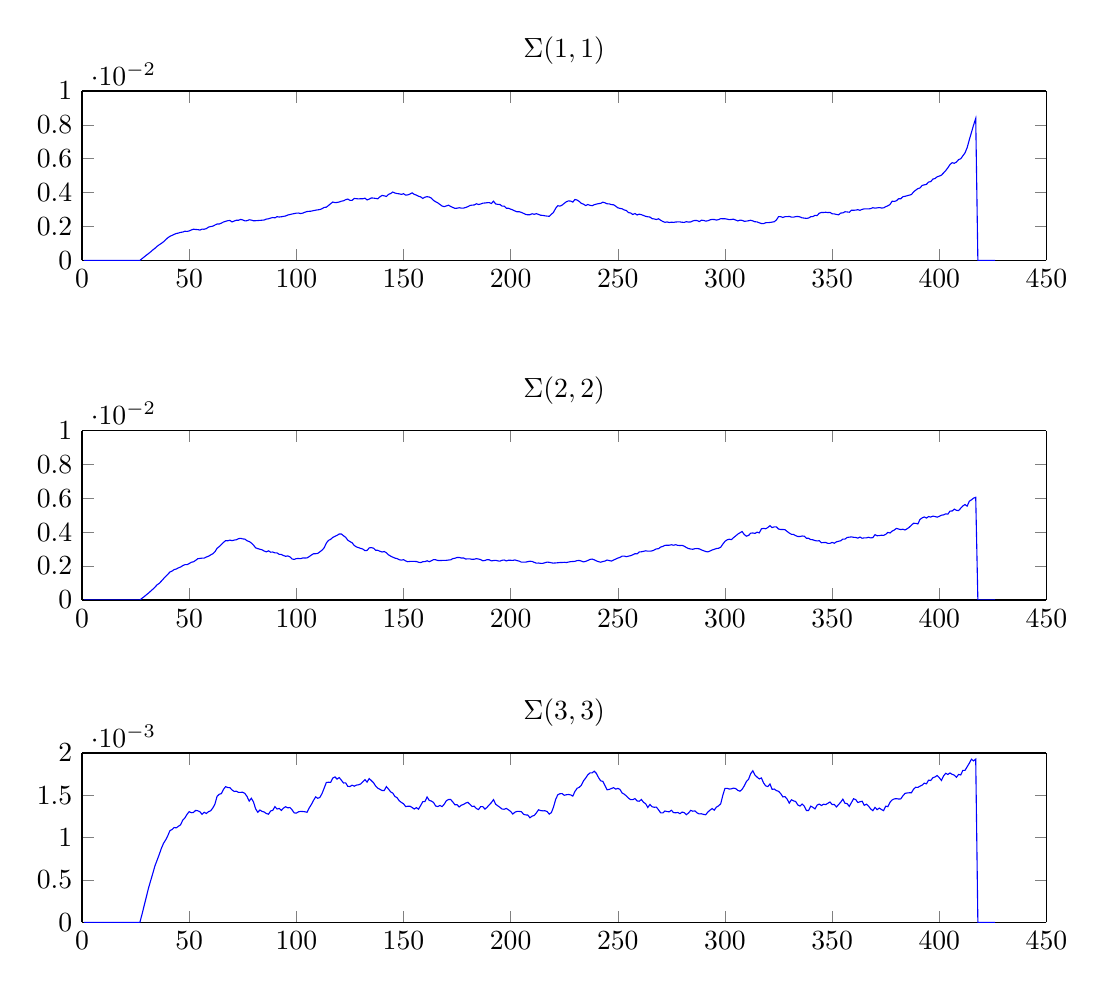
\begin{tikzpicture}

\begin{axis}[%
width=4.822in,
height=0.847in,
at={(0.809in,3.31in)},
scale only axis,
separate axis lines,
every outer x axis line/.append style={black},
every x tick label/.append style={font=\color{black}},
xmin=0,
xmax=450,
every outer y axis line/.append style={black},
every y tick label/.append style={font=\color{black}},
ymin=0,
ymax=0.01,
axis background/.style={fill=white},
title={$\Sigma\text{(1,1)}$}
]
\addplot [color=blue,solid,forget plot]
  table[row sep=crcr]{%
1	0\\
2	0\\
3	0\\
4	0\\
5	0\\
6	0\\
7	0\\
8	0\\
9	0\\
10	0\\
11	0\\
12	0\\
13	0\\
14	0\\
15	0\\
16	0\\
17	0\\
18	0\\
19	0\\
20	1.10668068063497e-28\\
21	6.1269188077788e-29\\
22	1.21154341531275e-27\\
23	2.16417281386742e-27\\
24	6.14431246491431e-27\\
25	6.28434927927247e-27\\
26	6.73213425124081e-27\\
27	5.07990940394863e-28\\
28	0.000100848759663641\\
29	0.00020187458630563\\
30	0.000305214346819941\\
31	0.000398660148707806\\
32	0.000499726900089777\\
33	0.00061192158000982\\
34	0.000708930345163692\\
35	0.000827918770452437\\
36	0.00091868681683618\\
37	0.00100197044500345\\
38	0.00109437218641779\\
39	0.00121342497173134\\
40	0.00133195545626767\\
41	0.00141823104363627\\
42	0.00147534380135983\\
43	0.00153731462564227\\
44	0.00158465558470437\\
45	0.00161161690715752\\
46	0.00165206093191761\\
47	0.00166981777931582\\
48	0.00171804000766001\\
49	0.00170631699294439\\
50	0.00173851789157291\\
51	0.00179223648974585\\
52	0.00183936471620231\\
53	0.00182310648097971\\
54	0.00181498429416863\\
55	0.00178917674870309\\
56	0.00183994667323329\\
57	0.00183880120246031\\
58	0.00187236753121147\\
59	0.00196158996028609\\
60	0.00199432071828742\\
61	0.00201714297453399\\
62	0.00208460294759297\\
63	0.00214652306975963\\
64	0.00214265193310957\\
65	0.00219868508884968\\
66	0.00226426280496353\\
67	0.00230408818126919\\
68	0.0023408784342245\\
69	0.00235403209879532\\
70	0.00226827797836073\\
71	0.00232033446250976\\
72	0.00236911589104423\\
73	0.002365903289477\\
74	0.0024171892358195\\
75	0.00238586112474731\\
76	0.00232927765645765\\
77	0.00234149551120929\\
78	0.00239405169022441\\
79	0.00237777287871326\\
80	0.00233320489064618\\
81	0.00234151787734478\\
82	0.00234948408204308\\
83	0.00235944604561368\\
84	0.0023699385354519\\
85	0.00238191501583074\\
86	0.00243532228243168\\
87	0.00245332531953899\\
88	0.00249787718767231\\
89	0.00252682422052829\\
90	0.00251095190728026\\
91	0.00257744077134686\\
92	0.00255862456799322\\
93	0.00257329973758199\\
94	0.0025964145974395\\
95	0.00261983730191888\\
96	0.00267576439870782\\
97	0.00270363472710814\\
98	0.00273540525674294\\
99	0.00276067516512187\\
100	0.00278631074366188\\
101	0.00279233327817584\\
102	0.00276275022841953\\
103	0.00278865765676907\\
104	0.00284144709007201\\
105	0.00288280220871039\\
106	0.00289431325542503\\
107	0.0029046595732406\\
108	0.00293621878515766\\
109	0.00296127253800892\\
110	0.00298144365824422\\
111	0.00300197408752758\\
112	0.00304853956320662\\
113	0.00312738246397327\\
114	0.00313752844144664\\
115	0.00323995894700459\\
116	0.00334426486425147\\
117	0.00344330092484347\\
118	0.00340927013385469\\
119	0.00341733958671464\\
120	0.00344580903204775\\
121	0.00349192413918856\\
122	0.00351637763763639\\
123	0.00358221663619034\\
124	0.00361705091063439\\
125	0.0035436681607256\\
126	0.00354119616168422\\
127	0.0036529348867921\\
128	0.00364123727188945\\
129	0.003626852367933\\
130	0.00363783043905127\\
131	0.00363251396216881\\
132	0.00367344457001959\\
133	0.00356800291719922\\
134	0.00361325887447694\\
135	0.00368506220515819\\
136	0.00367453225551926\\
137	0.00365665373707\\
138	0.00363466810309075\\
139	0.0037509007557095\\
140	0.00383212035603466\\
141	0.00380973917925498\\
142	0.0037728854319384\\
143	0.00389388972526819\\
144	0.00394511636830079\\
145	0.00403256666484179\\
146	0.00397428300900783\\
147	0.00394277203690242\\
148	0.0039267521983077\\
149	0.00389409260409789\\
150	0.00393183027997855\\
151	0.00385070532229674\\
152	0.00386387169272818\\
153	0.00391435810966989\\
154	0.00398516930076559\\
155	0.00389521188821937\\
156	0.00385464520089499\\
157	0.00378587264207597\\
158	0.00374943798269655\\
159	0.00365622475233085\\
160	0.00373113035666882\\
161	0.00375880836109623\\
162	0.00373744149184959\\
163	0.00367190667563139\\
164	0.0035382154659741\\
165	0.00346171558808308\\
166	0.00339279018079965\\
167	0.00329994637304831\\
168	0.00320698079219232\\
169	0.00316911963246575\\
170	0.00321136256350379\\
171	0.00325581854841401\\
172	0.00318083539976905\\
173	0.00312403689446414\\
174	0.00306927534170966\\
175	0.00307801036982269\\
176	0.0031067814948014\\
177	0.00308267425073142\\
178	0.00308521063868562\\
179	0.00312071836267238\\
180	0.00316907108981676\\
181	0.00323735917622743\\
182	0.00326140044617571\\
183	0.0032669441160519\\
184	0.00334048681538286\\
185	0.00329794248103543\\
186	0.00332671759036052\\
187	0.00337396268442482\\
188	0.00338666859837515\\
189	0.00340301556506458\\
190	0.00341065571121403\\
191	0.00335540547875238\\
192	0.00349252741341112\\
193	0.00333132426594948\\
194	0.00330207179669148\\
195	0.0032985388514196\\
196	0.00320242889181633\\
197	0.00319601154911751\\
198	0.00307514549851362\\
199	0.00307477024042898\\
200	0.00302247293532463\\
201	0.00297537751101938\\
202	0.00291477690550335\\
203	0.00286461940120865\\
204	0.00287415118853271\\
205	0.0028301426446641\\
206	0.00277349706618181\\
207	0.00271072448634254\\
208	0.00268867243669324\\
209	0.00269340681839635\\
210	0.00275209560572301\\
211	0.00271741746342264\\
212	0.00275733382987517\\
213	0.00271144055892187\\
214	0.00266378446039729\\
215	0.00265237171957067\\
216	0.00262965062063816\\
217	0.00261164909910056\\
218	0.00260043668310072\\
219	0.00272049309242529\\
220	0.00283304822372427\\
221	0.00307734942174367\\
222	0.00322628078786898\\
223	0.00320004568578852\\
224	0.00326173375686092\\
225	0.00336393498011407\\
226	0.00345820530964664\\
227	0.00351023494096158\\
228	0.00349817005547822\\
229	0.00343877432271297\\
230	0.00359610133657647\\
231	0.00355797273417922\\
232	0.0034777240401972\\
233	0.00336273886208658\\
234	0.00331824633399705\\
235	0.0032336949960527\\
236	0.00329751175641192\\
237	0.00325012762354946\\
238	0.00322694639863512\\
239	0.00328326790187974\\
240	0.00331957731045358\\
241	0.00334860372720795\\
242	0.00336579111464971\\
243	0.0034328540094083\\
244	0.00339741840515641\\
245	0.00333921638153673\\
246	0.003335385397944\\
247	0.00328980350271625\\
248	0.00328045930314612\\
249	0.00320126414066233\\
250	0.00310218241601566\\
251	0.00306779083494196\\
252	0.00304420443128089\\
253	0.00297414233423904\\
254	0.00294143314650612\\
255	0.00281809131033094\\
256	0.00279642880777856\\
257	0.00270547362033571\\
258	0.00276381895253267\\
259	0.00267810717498941\\
260	0.00272767925454094\\
261	0.0026955688712623\\
262	0.00264957642035699\\
263	0.00259856800007769\\
264	0.00257361222452978\\
265	0.00255657640871781\\
266	0.00246215825353807\\
267	0.00244395477210011\\
268	0.00241164645240594\\
269	0.00245530732164177\\
270	0.00236710289468012\\
271	0.00229530405959478\\
272	0.00224568073416289\\
273	0.00226659077539502\\
274	0.00223464330375853\\
275	0.00225210003804218\\
276	0.00224238070355001\\
277	0.00226239299895728\\
278	0.00227047348998711\\
279	0.0022678346304781\\
280	0.00224832191366107\\
281	0.00224248960935349\\
282	0.00228144221268781\\
283	0.00225891346326784\\
284	0.00226779203284323\\
285	0.00232571324196953\\
286	0.00235590248557222\\
287	0.00234883423819427\\
288	0.00228787734448393\\
289	0.00236858726750108\\
290	0.00235776727640733\\
291	0.00231465683392346\\
292	0.00233598980586208\\
293	0.00238979528474089\\
294	0.00241612506176601\\
295	0.00241167162108977\\
296	0.00237699012969247\\
297	0.00240517524894465\\
298	0.00246111690188362\\
299	0.00245687120641529\\
300	0.00245554727911624\\
301	0.00243295940622249\\
302	0.00240148171280924\\
303	0.0024140663616195\\
304	0.00243143879798746\\
305	0.00237844958476717\\
306	0.00232819459928758\\
307	0.00237307907753375\\
308	0.00236189148596975\\
309	0.00230589615424601\\
310	0.00231493988663886\\
311	0.00233900216899811\\
312	0.00236657304854402\\
313	0.00232764349488959\\
314	0.00227842531811331\\
315	0.00227146495343276\\
316	0.00221412839590192\\
317	0.0021764469820796\\
318	0.00216589780628802\\
319	0.00222209450781776\\
320	0.00222598152870172\\
321	0.00223784271737126\\
322	0.00225659156987155\\
323	0.0022810933586937\\
324	0.00238604252196671\\
325	0.00258002512752241\\
326	0.00257839317942149\\
327	0.00253273937677315\\
328	0.00257676885317372\\
329	0.00257966222034914\\
330	0.00259304067974815\\
331	0.00255238637078959\\
332	0.0025514472362451\\
333	0.00258285827787676\\
334	0.00258995261429763\\
335	0.0025645178523464\\
336	0.00251067566123136\\
337	0.00249401033119698\\
338	0.00247790409138355\\
339	0.00249788883940928\\
340	0.00257434198523513\\
341	0.00258575158695108\\
342	0.00265603210934583\\
343	0.00264462156415792\\
344	0.00278446326520044\\
345	0.00282585908575521\\
346	0.00282289573351223\\
347	0.0028401094606798\\
348	0.00282000928241824\\
349	0.00283092890285192\\
350	0.00274998437542993\\
351	0.00274003754852565\\
352	0.00271131781225898\\
353	0.00268886344780581\\
354	0.00279143233929278\\
355	0.00280323697581848\\
356	0.00286998274023674\\
357	0.00285703282056481\\
358	0.00284092053650496\\
359	0.00295589296472323\\
360	0.00295744649833703\\
361	0.00296470154287788\\
362	0.00299412335421933\\
363	0.00295230576426795\\
364	0.00301133810426407\\
365	0.00303797344449657\\
366	0.00304132025756168\\
367	0.00303499572730093\\
368	0.00305693595326837\\
369	0.00310822968073136\\
370	0.00308137675693312\\
371	0.00309829259605997\\
372	0.00311597387892222\\
373	0.00309151746079285\\
374	0.00309520155722467\\
375	0.00316952145388568\\
376	0.00321903484475224\\
377	0.00329925077708536\\
378	0.00349103613942927\\
379	0.00347746133843664\\
380	0.00351660771752692\\
381	0.00363790133883498\\
382	0.00363399260403543\\
383	0.00375810841157792\\
384	0.00378019550220131\\
385	0.00381531438437427\\
386	0.00384959868468275\\
387	0.00388705878373685\\
388	0.00403860588816837\\
389	0.00414604309088629\\
390	0.0042334946587986\\
391	0.00427367079910944\\
392	0.00442306181322667\\
393	0.00445673700429629\\
394	0.00448589268786409\\
395	0.00462184171616086\\
396	0.00464834394488013\\
397	0.00479597851303637\\
398	0.00483192938404075\\
399	0.00492840165468948\\
400	0.00497465682900664\\
401	0.0050301619736226\\
402	0.00516281013157313\\
403	0.0052994938873196\\
404	0.00546464233796071\\
405	0.00565770158380136\\
406	0.00576519648909404\\
407	0.00573169884412423\\
408	0.00580283648877756\\
409	0.00594635015888821\\
410	0.00599745319912589\\
411	0.00617058143416695\\
412	0.00634555457321202\\
413	0.00665201162897187\\
414	0.00711568500770019\\
415	0.00754824961331814\\
416	0.00798618136175051\\
417	0.00838168466761682\\
418	0\\
419	8.59482111715421e-29\\
420	4.52065586738225e-28\\
421	5.69824097157236e-28\\
422	5.2058007742508e-28\\
423	1.15426823496841e-27\\
424	3.32046270707128e-27\\
425	1.33844130021813e-26\\
426	1.32562719207329e-26\\
};
\end{axis}

\begin{axis}[%
width=4.822in,
height=0.847in,
at={(0.809in,1.612in)},
scale only axis,
separate axis lines,
every outer x axis line/.append style={black},
every x tick label/.append style={font=\color{black}},
xmin=0,
xmax=450,
every outer y axis line/.append style={black},
every y tick label/.append style={font=\color{black}},
ymin=0,
ymax=0.01,
axis background/.style={fill=white},
title={$\Sigma\text{(2,2)}$}
]
\addplot [color=blue,solid,forget plot]
  table[row sep=crcr]{%
1	0\\
2	0\\
3	0\\
4	0\\
5	0\\
6	0\\
7	0\\
8	0\\
9	0\\
10	0\\
11	0\\
12	0\\
13	0\\
14	0\\
15	0\\
16	0\\
17	0\\
18	0\\
19	0\\
20	2.3092102757602e-31\\
21	3.44565267984446e-32\\
22	7.56912744955378e-31\\
23	1.74978076984088e-30\\
24	6.07704005843463e-30\\
25	3.31726457317823e-31\\
26	1.06904617200073e-30\\
27	5.7604983688661e-33\\
28	9.9706112770798e-05\\
29	0.000195264961901317\\
30	0.000302657841997122\\
31	0.000403140083555271\\
32	0.00051829659432825\\
33	0.000630224393405465\\
34	0.000753061453319728\\
35	0.000889588761697916\\
36	0.000976179111015932\\
37	0.001110031024608\\
38	0.00125017646731135\\
39	0.00138873757680387\\
40	0.00150979479602322\\
41	0.0016481467399085\\
42	0.00170400928396534\\
43	0.00179305297270795\\
44	0.00182790202676668\\
45	0.00189478946880596\\
46	0.00194497810609458\\
47	0.00202820008269657\\
48	0.00208224033899094\\
49	0.00208357650600246\\
50	0.00214745474228115\\
51	0.00222496606119348\\
52	0.00225243853589112\\
53	0.0023360365409956\\
54	0.00243288596155356\\
55	0.00245216652863957\\
56	0.00246858645113004\\
57	0.00246712412777587\\
58	0.00253511828966251\\
59	0.00258122615058212\\
60	0.00265780429982336\\
61	0.00272347404857537\\
62	0.0028423659542254\\
63	0.00304547311890563\\
64	0.00314782465076192\\
65	0.0032698934847379\\
66	0.00339737473162562\\
67	0.00350108165764746\\
68	0.00349381816107716\\
69	0.00353211737004792\\
70	0.0035020092601733\\
71	0.00353360769701727\\
72	0.00355544247024938\\
73	0.00361688865341291\\
74	0.00363794022178958\\
75	0.00360303739151165\\
76	0.00359140594527181\\
77	0.00349332738508309\\
78	0.00344930550098657\\
79	0.00336176116363055\\
80	0.00323854779682972\\
81	0.00307591618251345\\
82	0.00303127498366353\\
83	0.00299217628538033\\
84	0.00296100663902265\\
85	0.00288841280644674\\
86	0.00283865219161244\\
87	0.00290055828510472\\
88	0.00281892979223406\\
89	0.00282931775579293\\
90	0.00277961036784225\\
91	0.0027746785115651\\
92	0.00269414072519423\\
93	0.00268365942301006\\
94	0.00262127966336223\\
95	0.002576220549711\\
96	0.00259994826931097\\
97	0.00254387052982565\\
98	0.00241812919549748\\
99	0.00239283704734936\\
100	0.00244112122472041\\
101	0.00244775481621803\\
102	0.00243700696470546\\
103	0.00248091555193516\\
104	0.00247615170126388\\
105	0.00248183172696894\\
106	0.00255946216754186\\
107	0.00264930639126633\\
108	0.00272638216404524\\
109	0.0027305429792762\\
110	0.00274998690728484\\
111	0.00284309636369812\\
112	0.00293887166051347\\
113	0.00308285745581302\\
114	0.00335942662762876\\
115	0.00351724898962991\\
116	0.00357880020417161\\
117	0.00369253156340483\\
118	0.00375549352465571\\
119	0.00381358692416067\\
120	0.00389445764591422\\
121	0.00389604900819425\\
122	0.00378992290215619\\
123	0.00369579866579864\\
124	0.00352827373246085\\
125	0.00344671395140915\\
126	0.00337690448854643\\
127	0.00321730109195499\\
128	0.00313190468035931\\
129	0.00308890906856404\\
130	0.00304314152992045\\
131	0.00300688661547937\\
132	0.00291114719341054\\
133	0.00292340467326134\\
134	0.00307548364257663\\
135	0.00308950290906321\\
136	0.00305438130803266\\
137	0.00293619419997882\\
138	0.00293068496821192\\
139	0.00287200271735087\\
140	0.00282955633375852\\
141	0.00285829269471127\\
142	0.00278746640545434\\
143	0.00266462485274948\\
144	0.00258821366906306\\
145	0.00252644037984459\\
146	0.00246883414171643\\
147	0.00244005744020341\\
148	0.0023757220215848\\
149	0.00235010153607885\\
150	0.00237926101073597\\
151	0.00230322310177544\\
152	0.00225812243697355\\
153	0.00227322962455555\\
154	0.00227460371364749\\
155	0.00227694802835216\\
156	0.00226765936658114\\
157	0.00222593997947298\\
158	0.00220363815398156\\
159	0.00225766055065618\\
160	0.00225995378292404\\
161	0.0023125352988197\\
162	0.0022583829667902\\
163	0.00231217019899345\\
164	0.00238185811571108\\
165	0.0023729202529566\\
166	0.0023284583159521\\
167	0.00232545369819298\\
168	0.00233220064592596\\
169	0.00233919888782922\\
170	0.00233985819719473\\
171	0.00235679734898935\\
172	0.00236800329116648\\
173	0.00243787100235458\\
174	0.00246161400309037\\
175	0.00250443351809805\\
176	0.00250999567774871\\
177	0.00247312227055276\\
178	0.00247866689410863\\
179	0.00241691964593458\\
180	0.00242536754635025\\
181	0.00242202139110883\\
182	0.00239809540404968\\
183	0.0024047810593772\\
184	0.00243863367377085\\
185	0.00241484681024189\\
186	0.00238423645677218\\
187	0.00231257693651683\\
188	0.00232952772379446\\
189	0.0023778307825746\\
190	0.00237170936776238\\
191	0.00230654824128771\\
192	0.00232733862132599\\
193	0.00233658431451234\\
194	0.00230788530019295\\
195	0.00228994276805879\\
196	0.00234387563245129\\
197	0.00235784020423919\\
198	0.00230451211977211\\
199	0.00234771210514634\\
200	0.00234163028300735\\
201	0.00233596592582212\\
202	0.00236084623294768\\
203	0.0023216969304872\\
204	0.00229272557257355\\
205	0.00222947841904866\\
206	0.00223212337837299\\
207	0.00223128377534369\\
208	0.0022631263320157\\
209	0.00228463950739984\\
210	0.0022741239343279\\
211	0.00221818203430041\\
212	0.00217224400988498\\
213	0.00217931035104218\\
214	0.0021609813749552\\
215	0.00215937306593518\\
216	0.00219911469073678\\
217	0.00223421724864596\\
218	0.00222145307186885\\
219	0.00219131245059122\\
220	0.00217492595607537\\
221	0.0021853352430007\\
222	0.00219658899924706\\
223	0.00220938224197246\\
224	0.00221125884431765\\
225	0.00222284242840037\\
226	0.00220904961417307\\
227	0.00223631456765684\\
228	0.00226319694318526\\
229	0.00226937420401831\\
230	0.00228084047208922\\
231	0.00232319699211223\\
232	0.00233095742191942\\
233	0.00229527966186581\\
234	0.00224574073829022\\
235	0.00227857264234822\\
236	0.00233120180447494\\
237	0.00239059721322884\\
238	0.00241415915939175\\
239	0.00236996473779623\\
240	0.00230386632798661\\
241	0.00226031858693508\\
242	0.00222847536476012\\
243	0.00226795996155498\\
244	0.00229609255827098\\
245	0.00235489372372258\\
246	0.0023252145676533\\
247	0.00229486835196553\\
248	0.00235669593761166\\
249	0.00241343357390411\\
250	0.00247130709940302\\
251	0.00251129432960098\\
252	0.00258521853390262\\
253	0.00258943952560804\\
254	0.00255317043034723\\
255	0.00258701477499137\\
256	0.00261569381602568\\
257	0.00266474167481027\\
258	0.00272868829969381\\
259	0.00272146028902216\\
260	0.00283253859032342\\
261	0.00284317873351517\\
262	0.00287053114334781\\
263	0.00290188978715412\\
264	0.0028798639587608\\
265	0.00288055228316175\\
266	0.00289643293680445\\
267	0.00294905174464496\\
268	0.00301389157171348\\
269	0.00302715452730709\\
270	0.00312330397422029\\
271	0.00315910336899373\\
272	0.00322431875266177\\
273	0.00322924930027064\\
274	0.00323064168070766\\
275	0.00325873457078564\\
276	0.00323071136591582\\
277	0.00325966892431472\\
278	0.00322251603580097\\
279	0.00321318711078771\\
280	0.0032196893873097\\
281	0.00317167987845344\\
282	0.00309512546691343\\
283	0.00303294483271509\\
284	0.00300802973329726\\
285	0.00299166345312673\\
286	0.00302929382591735\\
287	0.00303570138826785\\
288	0.00301742010863037\\
289	0.00295505117839523\\
290	0.00290818363941257\\
291	0.00285982384431352\\
292	0.002837123233782\\
293	0.00288920328862201\\
294	0.00294807233697439\\
295	0.00299029940659347\\
296	0.00303410287777665\\
297	0.00305194519150872\\
298	0.00310972708048728\\
299	0.0032964556726566\\
300	0.00346136833407191\\
301	0.00354928384118447\\
302	0.00358488126525837\\
303	0.003561975798834\\
304	0.00367779350868468\\
305	0.00378127002167373\\
306	0.00388720290216018\\
307	0.00396445934544959\\
308	0.00403950043191575\\
309	0.00386108247025581\\
310	0.00376374225286592\\
311	0.00380625784352414\\
312	0.00394111004883109\\
313	0.00395509937028042\\
314	0.00392805100446453\\
315	0.00400133641774484\\
316	0.00395976213864897\\
317	0.00419860010570251\\
318	0.00422544015641185\\
319	0.00420415757598269\\
320	0.0042756260447922\\
321	0.00438656332995888\\
322	0.00427045940765805\\
323	0.00431285330144758\\
324	0.00431289132797253\\
325	0.0041868155656308\\
326	0.00415891649256709\\
327	0.00416186628365365\\
328	0.00414548218320255\\
329	0.00404478094513689\\
330	0.00394904939613886\\
331	0.00387736879529139\\
332	0.00386300653877788\\
333	0.00379732173417042\\
334	0.0037449876156864\\
335	0.00374414465402782\\
336	0.00377596243031467\\
337	0.0037601461021554\\
338	0.00364422151271013\\
339	0.00363973826078994\\
340	0.00356246272328352\\
341	0.00355374538510005\\
342	0.00350467261822647\\
343	0.00348273015103891\\
344	0.00349870422617835\\
345	0.00337945298657171\\
346	0.00338949327166686\\
347	0.00339529520410932\\
348	0.00333888106451753\\
349	0.00334027918310603\\
350	0.00339889679870949\\
351	0.00334667740122978\\
352	0.00343052242300892\\
353	0.0034642584103535\\
354	0.00349270633761521\\
355	0.00359122078594816\\
356	0.00359368192347755\\
357	0.00368873948826739\\
358	0.0037055021742321\\
359	0.00372382329111147\\
360	0.00369827565194334\\
361	0.00368896114877588\\
362	0.00364880138896306\\
363	0.00371150438425152\\
364	0.00364333427910132\\
365	0.0036666582262105\\
366	0.00366640129348994\\
367	0.00369895144776376\\
368	0.00366369542100663\\
369	0.00367980893194507\\
370	0.00385166228073988\\
371	0.00379125981297013\\
372	0.00379806748901771\\
373	0.00382335666031338\\
374	0.00380884546591918\\
375	0.00387004191230176\\
376	0.00398646242430437\\
377	0.00395330537772604\\
378	0.0040635479513641\\
379	0.00413016327025163\\
380	0.00422528825682075\\
381	0.00418720632412052\\
382	0.00415309375921787\\
383	0.00417624376685373\\
384	0.00413095988073406\\
385	0.00420282255245611\\
386	0.00429326361903746\\
387	0.00441636105790642\\
388	0.00452572949470859\\
389	0.00452311998558726\\
390	0.00448943839291785\\
391	0.0047533746644874\\
392	0.0048436515065178\\
393	0.00490257622303824\\
394	0.00483300549325316\\
395	0.00492312944767602\\
396	0.00489198333067738\\
397	0.00494982389003544\\
398	0.00492456934547167\\
399	0.00488698701401681\\
400	0.00493761899522503\\
401	0.00500470304373184\\
402	0.00501969436244894\\
403	0.00508172347060684\\
404	0.00506466769840807\\
405	0.00524724051860508\\
406	0.00524861406530765\\
407	0.00536040213244758\\
408	0.00529440837203149\\
409	0.00527200847254663\\
410	0.00541604507277243\\
411	0.00555130118675692\\
412	0.00563144729927447\\
413	0.00553815090040565\\
414	0.00582399302661987\\
415	0.00590824257405288\\
416	0.0060119094672407\\
417	0.00605715281419544\\
418	0\\
419	2.91088280939153e-31\\
420	8.20058716756694e-31\\
421	7.05430649061133e-30\\
422	4.43778637050524e-31\\
423	7.28507703986261e-31\\
424	7.91782033798578e-30\\
425	3.47146272210348e-30\\
426	8.49420047479519e-32\\
};
\end{axis}

\begin{axis}[%
width=4.822in,
height=0.847in,
at={(0.809in,0in)},
scale only axis,
separate axis lines,
every outer x axis line/.append style={black},
every x tick label/.append style={font=\color{black}},
xmin=0,
xmax=450,
every outer y axis line/.append style={black},
every y tick label/.append style={font=\color{black}},
ymin=0,
ymax=0.002,
axis background/.style={fill=white},
title={$\Sigma\text{(3,3)}$}
]
\addplot [color=blue,solid,forget plot]
  table[row sep=crcr]{%
1	0\\
2	0\\
3	0\\
4	0\\
5	0\\
6	0\\
7	0\\
8	0\\
9	0\\
10	0\\
11	0\\
12	0\\
13	0\\
14	0\\
15	0\\
16	0\\
17	0\\
18	0\\
19	0\\
20	1.7248535839131e-29\\
21	1.06370118190604e-31\\
22	2.76784112346234e-30\\
23	3.13115298114261e-32\\
24	1.72462907025259e-30\\
25	5.12096548873076e-35\\
26	4.44279729871901e-30\\
27	6.81895538115503e-31\\
28	9.6754161160143e-05\\
29	0.000199203365673765\\
30	0.000299806152315689\\
31	0.000403208800830536\\
32	0.000490283724806267\\
33	0.000575907031529369\\
34	0.000665539780286951\\
35	0.000731959078140335\\
36	0.000800034334701908\\
37	0.000872365582738991\\
38	0.000932074499517547\\
39	0.000972110181864041\\
40	0.0010215964353307\\
41	0.00108218939916819\\
42	0.00109647367839539\\
43	0.00111947447430318\\
44	0.00111559815320495\\
45	0.00113515870536039\\
46	0.00115224211143195\\
47	0.00120757881927716\\
48	0.00123340289242875\\
49	0.0012761707792227\\
50	0.00130666509103807\\
51	0.00129458709535377\\
52	0.0012975532555746\\
53	0.00132179407519462\\
54	0.00131734114049655\\
55	0.00130570929149467\\
56	0.00127573212231027\\
57	0.00129903417089321\\
58	0.00128592061881932\\
59	0.00130640921475655\\
60	0.00131710618613246\\
61	0.00134909121622021\\
62	0.00139580420987756\\
63	0.00148717668624035\\
64	0.00151142977211426\\
65	0.00151987126692867\\
66	0.00157026660614571\\
67	0.00160209280477698\\
68	0.00159169870077908\\
69	0.00159019406284468\\
70	0.00156287000211426\\
71	0.00154547201879725\\
72	0.00154847670973836\\
73	0.0015341753835482\\
74	0.00153517435948171\\
75	0.00153585471545436\\
76	0.00152176027045775\\
77	0.00148533875684316\\
78	0.0014311380805345\\
79	0.00146475970301018\\
80	0.00142174733901931\\
81	0.00134015761242633\\
82	0.00130016611276461\\
83	0.0013255428184455\\
84	0.00131030773020504\\
85	0.0013024266197457\\
86	0.00128485267482426\\
87	0.00127647015690003\\
88	0.00131496140986789\\
89	0.00132210355481093\\
90	0.00136593566145524\\
91	0.00133785161424463\\
92	0.00134503922090162\\
93	0.00132170603841747\\
94	0.00134839921650332\\
95	0.00136520428968119\\
96	0.00135163911024807\\
97	0.00135564293542188\\
98	0.00132886137726828\\
99	0.00129206828327547\\
100	0.00128955426013171\\
101	0.0013052585128418\\
102	0.00130991570672195\\
103	0.00130849676081887\\
104	0.00130590946919857\\
105	0.00129936972832147\\
106	0.0013507386769909\\
107	0.00139109213404748\\
108	0.00143965546460088\\
109	0.00148096330768914\\
110	0.00146428398498244\\
111	0.00147586135058393\\
112	0.00152164465639154\\
113	0.00158557225756186\\
114	0.00165171443338191\\
115	0.00165408533320084\\
116	0.00165259869069844\\
117	0.00170432941931576\\
118	0.00171714100719894\\
119	0.00169167719164948\\
120	0.00170953945129422\\
121	0.00167840771666489\\
122	0.00164567527601362\\
123	0.00164681635722947\\
124	0.00160600985742446\\
125	0.00160324713803425\\
126	0.0016195001247134\\
127	0.00160778147571387\\
128	0.0016205478776052\\
129	0.00162400448859259\\
130	0.00163381770169068\\
131	0.00165939601009028\\
132	0.0016852147883562\\
133	0.00165589770624522\\
134	0.0016979890936276\\
135	0.0016733481602648\\
136	0.00164868130539554\\
137	0.00160897071398567\\
138	0.00158327113456202\\
139	0.00157065072261171\\
140	0.00155631864410361\\
141	0.00155659827931927\\
142	0.00160220800657783\\
143	0.00157369798710519\\
144	0.0015401161184108\\
145	0.00152560782405799\\
146	0.00148618071603048\\
147	0.00147160447652702\\
148	0.00143591223622855\\
149	0.00141572051093514\\
150	0.00140078659832657\\
151	0.00136641525408019\\
152	0.0013710756899813\\
153	0.00137138087119164\\
154	0.00135674775378257\\
155	0.00133792195564667\\
156	0.00135456606494152\\
157	0.00133587200199145\\
158	0.00137964408404113\\
159	0.00142441754332339\\
160	0.00142537524220168\\
161	0.00147983716143466\\
162	0.00143996537219037\\
163	0.00143230112941062\\
164	0.0014156584793652\\
165	0.0013737215884038\\
166	0.00136741147589617\\
167	0.00138017437325064\\
168	0.00136691925905098\\
169	0.00139466847124538\\
170	0.00143622177820473\\
171	0.00145000914069281\\
172	0.00145057609314006\\
173	0.00142168580788672\\
174	0.00138821728963338\\
175	0.00138790663381407\\
176	0.00136231288529131\\
177	0.00138367704835762\\
178	0.00139223832435803\\
179	0.0014079183682643\\
180	0.00141713960655984\\
181	0.001392706004028\\
182	0.00136814822424203\\
183	0.00137132348426966\\
184	0.00134315301043828\\
185	0.00133203676061731\\
186	0.00136647854691084\\
187	0.00136677333566025\\
188	0.00133676669587801\\
189	0.00135888101062154\\
190	0.00138746932026493\\
191	0.00141371055492804\\
192	0.00144916746773423\\
193	0.00139507477175163\\
194	0.00137609969991234\\
195	0.00135762741416442\\
196	0.0013376450138119\\
197	0.00133544184549174\\
198	0.00134538899183968\\
199	0.0013278948148298\\
200	0.0013091104691996\\
201	0.00127875693129451\\
202	0.00130086346685084\\
203	0.00130970269202077\\
204	0.0013095444015853\\
205	0.00130663163760585\\
206	0.0012765789714709\\
207	0.00126833336525075\\
208	0.00126682995134327\\
209	0.00123489278357952\\
210	0.00125414314656448\\
211	0.00126197245268243\\
212	0.0012925972889928\\
213	0.00132914431316953\\
214	0.00131980906065558\\
215	0.00131680535586316\\
216	0.00131731962241018\\
217	0.00130869452495883\\
218	0.00127815265425514\\
219	0.00129553536655735\\
220	0.00136237699861485\\
221	0.00145179698206201\\
222	0.00150652896302659\\
223	0.00151835300182406\\
224	0.00152045929747656\\
225	0.0015001369373442\\
226	0.00150636144914755\\
227	0.00151009719791592\\
228	0.00150465015167448\\
229	0.0014905641328116\\
230	0.00154590465811734\\
231	0.00158252763351101\\
232	0.0015949141855519\\
233	0.00161928599338058\\
234	0.00167139001050856\\
235	0.00170328831842226\\
236	0.0017416232573165\\
237	0.0017640090905657\\
238	0.00176480205455367\\
239	0.00178437701395232\\
240	0.00175860859200957\\
241	0.00170946115725696\\
242	0.0016709918951745\\
243	0.00166477697663183\\
244	0.00161576588458791\\
245	0.00156541843282333\\
246	0.00156950935529478\\
247	0.00158005833894228\\
248	0.0015904903247624\\
249	0.00157291576959621\\
250	0.00158170919193619\\
251	0.00156909492502477\\
252	0.00152788077674173\\
253	0.00151322823798498\\
254	0.00149195980772453\\
255	0.00146560133736168\\
256	0.00144828452575641\\
257	0.00144909447638486\\
258	0.00146139399869194\\
259	0.00143364846936791\\
260	0.001430030190862\\
261	0.00145031535645255\\
262	0.00141716287833444\\
263	0.00140015128906996\\
264	0.00135609407760717\\
265	0.00139157636703767\\
266	0.0013647395718138\\
267	0.0013590189349497\\
268	0.00136023358939131\\
269	0.0013281855690177\\
270	0.00129272295297476\\
271	0.00129182933470074\\
272	0.00131429970130774\\
273	0.00130828157434357\\
274	0.00130460619070009\\
275	0.00132338472153236\\
276	0.00129550697914511\\
277	0.00129363640644468\\
278	0.00129704418672982\\
279	0.00128304903132924\\
280	0.00130203528231314\\
281	0.001294819164506\\
282	0.00127168491139671\\
283	0.00129101604832138\\
284	0.00132185443718305\\
285	0.00131222392237511\\
286	0.00131561521049188\\
287	0.00129212943608748\\
288	0.00128061286316809\\
289	0.00128212675199019\\
290	0.00127434977384608\\
291	0.00127062624499807\\
292	0.00130184346880718\\
293	0.00132473362223438\\
294	0.00134341161701352\\
295	0.00132465040639261\\
296	0.00136066128057749\\
297	0.00137488752219386\\
298	0.00139969895879529\\
299	0.0015011951259519\\
300	0.00158191820352571\\
301	0.00158175544983102\\
302	0.0015737909218546\\
303	0.00157657556933595\\
304	0.00158486691619836\\
305	0.001579424598812\\
306	0.00155855256943751\\
307	0.00154834165696951\\
308	0.00157069786300814\\
309	0.00161139162282846\\
310	0.00166239126732431\\
311	0.00168907042854469\\
312	0.00175548914838796\\
313	0.00178979307942135\\
314	0.00173913392411074\\
315	0.00171445368336991\\
316	0.00169360040596805\\
317	0.00170514791963997\\
318	0.00164677372063768\\
319	0.00161107178592035\\
320	0.00160325542194868\\
321	0.00163362258667397\\
322	0.00157013343295921\\
323	0.00157397487788268\\
324	0.00155525310825572\\
325	0.00154741291936274\\
326	0.00152074108372628\\
327	0.00148088333556611\\
328	0.00148463315373839\\
329	0.00145513437374005\\
330	0.00140755316311721\\
331	0.00144731402016348\\
332	0.00143425800228531\\
333	0.00142631182167544\\
334	0.001385451354293\\
335	0.00137314380176544\\
336	0.00139686511639915\\
337	0.0013731329451762\\
338	0.00132104174386456\\
339	0.00131974822974635\\
340	0.00137143088873766\\
341	0.00135837583771851\\
342	0.0013393449641975\\
343	0.00138393922637382\\
344	0.0013960941205437\\
345	0.00137961452437825\\
346	0.00139459175686399\\
347	0.00139009327664205\\
348	0.00140579357735372\\
349	0.00142114124156016\\
350	0.00139050189855333\\
351	0.00139235087312719\\
352	0.00136239676076297\\
353	0.00139024445684926\\
354	0.00141884921472232\\
355	0.00145392856129467\\
356	0.00140630771175426\\
357	0.0014018805807347\\
358	0.00136857132517151\\
359	0.00141415178650178\\
360	0.00145929930736208\\
361	0.00144950856072683\\
362	0.00141479316290101\\
363	0.00142391818649302\\
364	0.0014299681730081\\
365	0.00138167585021859\\
366	0.00139513660050896\\
367	0.00137191035648503\\
368	0.00133821569349987\\
369	0.00131897055191841\\
370	0.00135738346231888\\
371	0.00133066780814565\\
372	0.00134899169013819\\
373	0.00133222416141408\\
374	0.00131887493750953\\
375	0.00137183470817798\\
376	0.00136545995510369\\
377	0.00141777369896475\\
378	0.00144540022832247\\
379	0.00145793885465185\\
380	0.00146038929838889\\
381	0.00145643723860481\\
382	0.00145705494076315\\
383	0.00149308074793898\\
384	0.00152222196317531\\
385	0.00152768882881863\\
386	0.00152977080074006\\
387	0.00153059332456909\\
388	0.00157262031408844\\
389	0.00159487909938003\\
390	0.00159290877129429\\
391	0.00160818588959097\\
392	0.00162020301812051\\
393	0.00164319411439647\\
394	0.00163563238867733\\
395	0.00167909650030264\\
396	0.00167477072965262\\
397	0.00170704626614322\\
398	0.00171686975426624\\
399	0.00173350706164378\\
400	0.00170776753742311\\
401	0.00167517200538889\\
402	0.00172942100306521\\
403	0.00175933991051307\\
404	0.00174619704098874\\
405	0.00176414798548735\\
406	0.0017471000031526\\
407	0.00173844307770727\\
408	0.00171279740762133\\
409	0.00174658899010658\\
410	0.00173993029513177\\
411	0.00179426208885431\\
412	0.0017946582568181\\
413	0.00183688442614995\\
414	0.00187873163670551\\
415	0.00192651237344538\\
416	0.00190647366048052\\
417	0.0019268923479514\\
418	0\\
419	1.77974025190453e-30\\
420	1.04053955816241e-30\\
421	4.88780684846589e-31\\
422	1.14438765963041e-29\\
423	7.32408102163463e-30\\
424	2.97487702750939e-29\\
425	5.76469219977654e-30\\
426	1.21735760886223e-30\\
};
\end{axis}
\end{tikzpicture}%}
	\caption{Uncertainties in pose for $M=1000$ (left) and $M=10000$ (right).}
	\label{fig:local_covariances_1000_10000}
\end{figure}


For the rest of the analysis we shall model stronger process noise with process noise and measurement covariance matrices $R,Q$:

	\[
	R =
	\begin{bmatrix}
	    5 		& 0		& 0 \\
	    0	    & 5		& 0 \\
	    0     	& 0 	& 1 \\
	
	\end{bmatrix}
	\]
	
	
	\[
	Q =
	\begin{bmatrix}
	    0.1  & 0 \\
	    0    & 0.1 \\
	
	\end{bmatrix}
	\]
	
	
In this map setting there are $4$ hypotheses, one for every landmark. Increasing the number of particles $M$ to $M=10000$ from $M=1000$ results
in these hypotheses being kept for longer and with more reliability. The main effect observed with a smaller number of particles is particle deprivation. This
effect is proportionally related to the level of process noise: the stronger the process noise, the less particle diversity is observed, hence the more
acute is the particle deprivation effect.

Regarding multinomial sampling, it is more or less evident that it is not as robust or reliable in preserving multiple hypotheses, since it introduces
sample variance and sequential sampling tackles this problem effectively.

Finally, the higher the measurement noise, the more spread-out are the particles around the hypotheses, which are still preserved, but with lower accuracy.
On the other hand, the lower the measurement noise, the less the degree in which the hypotheses are kept. When it reaches a certain threshold, we observe
no relation between the particle distribution and the given hypotheses.


\subsection{map\_sym3 $+$ so\_sym3\_nk}

Figure \ref{fig:pf_converge_10000} illustrates the convergence of the particle filter. Until timestep $t=180$ the upper right landmark has not been
observed, hence the robot keeps all $4$ hypotheses as to where it might be due to the symmetry of the $4$ landmarks it has seen. 
However, when it observes the $5^{th}$ landmark, this symmetry is resolved and it can reliably locate itself.


\begin{figure}
	\centering
	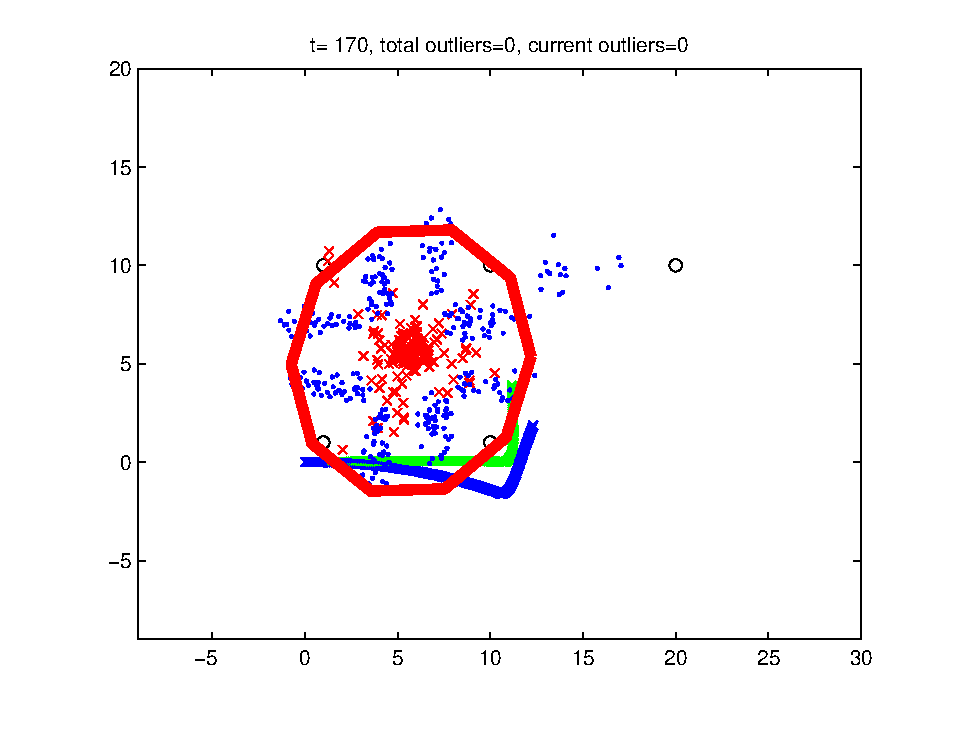
\includegraphics[scale=0.5]{./figures/M=10000/1.eps}
	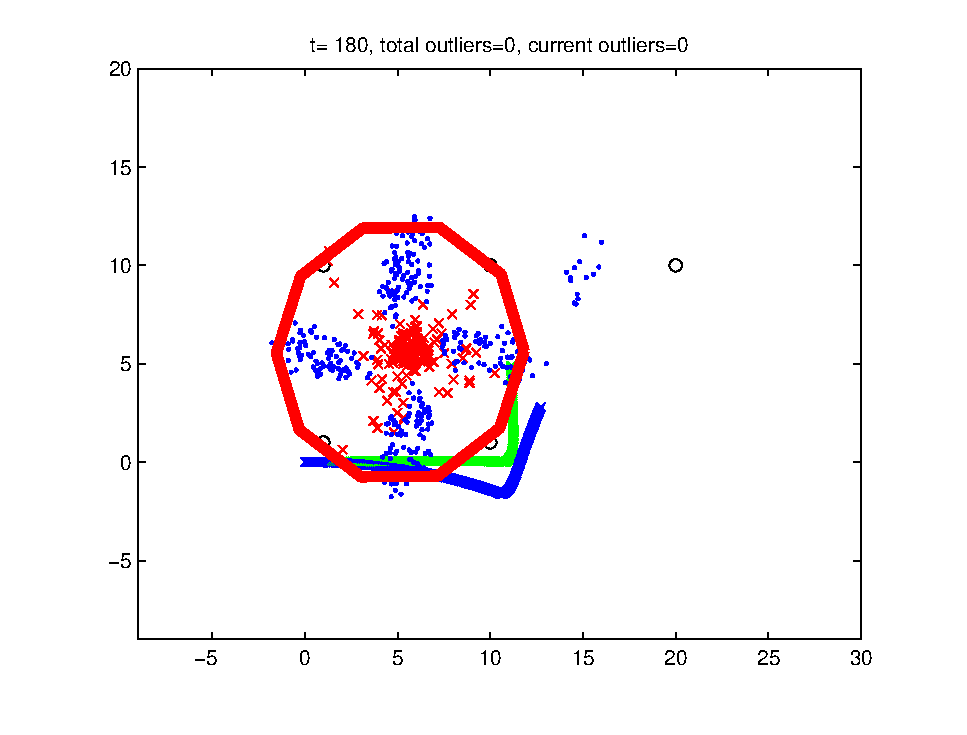
\includegraphics[scale=0.5]{./figures/M=10000/2.eps}
	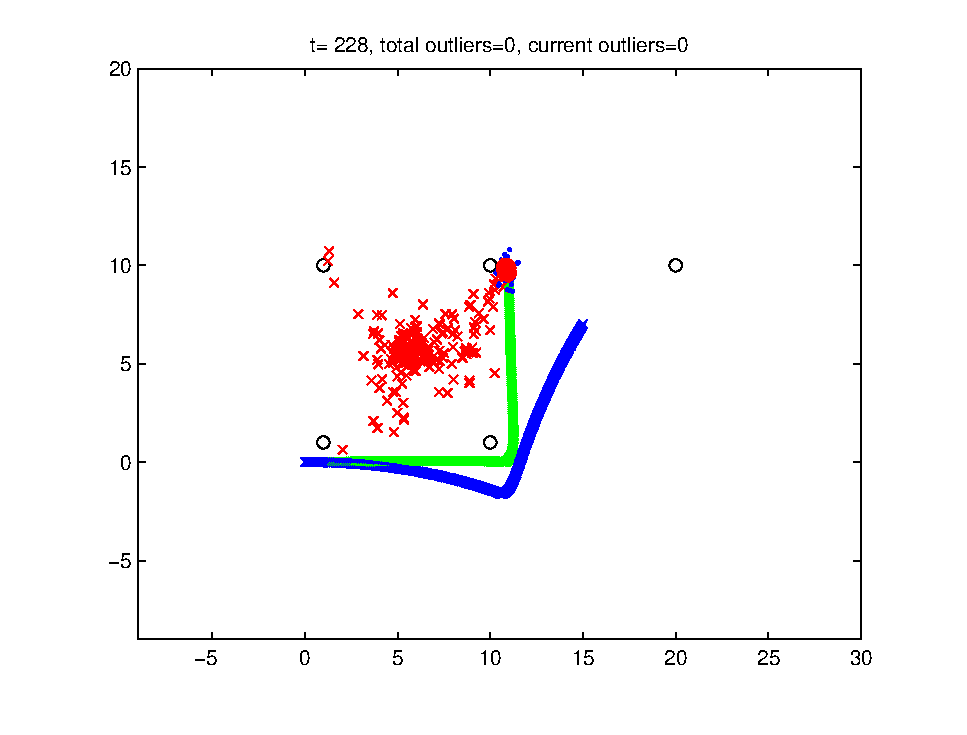
\includegraphics[scale=0.5]{./figures/M=10000/3.eps}
	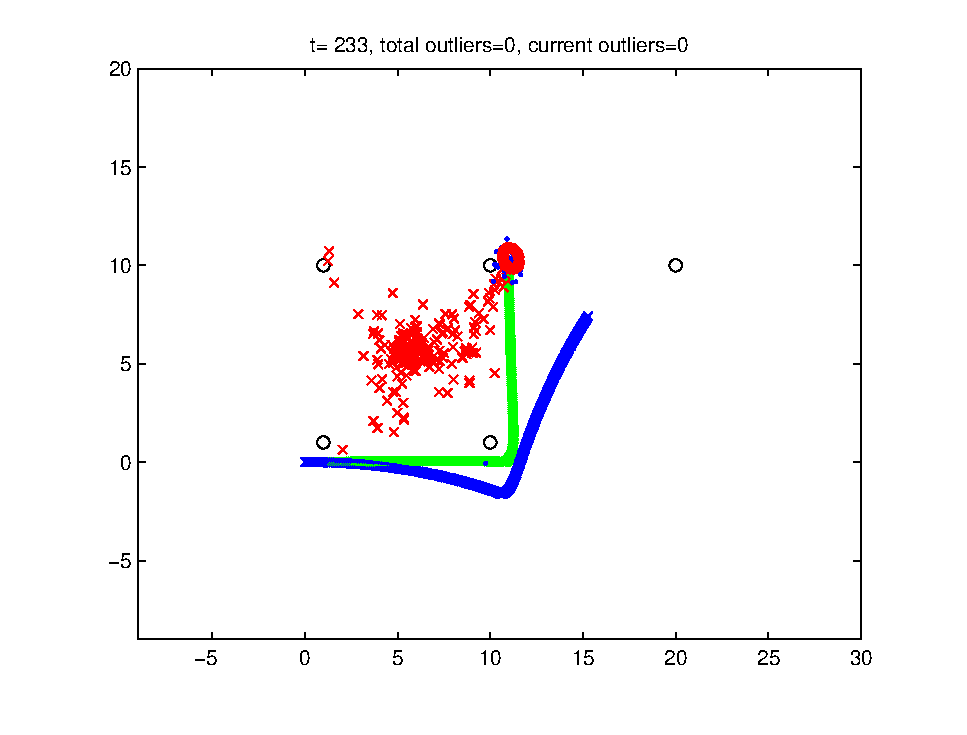
\includegraphics[scale=0.5]{./figures/M=10000/4.eps}
	\caption{Convergence of the PF to one single hypothesis due to symmetry resolution.}
	\label{fig:pf_converge_10000}
\end{figure}